\chapter{BDS and Final-Focus system as background sources}

\begin{chapterabstract}
 In this chapter, two of the sources for background at the interaction point (IP) coming directly from the Beam Delivery System (BDS) and the Final-Focus System (FF) are discussed: the background from beam halo collimators, and from muon spoilers.\\For the first, simulations with \bdsim were done, and data was taken at the ATF2 test bench facility where a new beam halo collimator was installed.\\For the latter, simulations with \mucarlo are shown, and the physics behind the background generation is explained.
\end{chapterabstract}


\section{Background from Beam Halo Collimators in the Final-Focus system}

The Final-Focus System (FF) is -as explained in Chapter~\ref{ILC}- responsible for focussing the beam to nanometre size. The reason behind this is the need for high luminosities which can be gained by small beam sizes. Another goal of the International Linear Collider is to have clean events with as little background as possible. A solution to this is to install beam halo collimators in the FF system that cut off the halo around the beam core. As the beam halo can interact with the beam pipe and its components, a beam halo collimation system plays an important role in the reduction of background at the IP. Nevertheless, the collimator itself can be source to particle showers and rises in the background level around the collimator location. Feasibility studies are needed to investigate in the effect of a beam halo collimator.\\
A vertical beam halo collimator was installed at the Accelerator Test Facility 2 (ATF2) at the research centre KEK in Japan. In March 2016, data of the background was taken with a Cherenkov detector in dependency of the aperture of this collimator at ATF2. This section covers the analysis of the data as well as the comparison of the data with simulations done with \bdsim. Both, the design of the vertical beam halo collimator at ATF2 and the \geant simulation tool \bdsim are explained here additionally.

\subsection{Beam Halo Collimator}
\label{Collimator}

The vertical beam halo collimator, for which the design drawings are shown in Figure~\ref{fig:collimator}, was installed in ATF2 in the beginning of March 2016. The collimating jaws are inside a structure that is evacuated and connected to the beam pipe of the ATF2 beam line. The actual jaws are made of Copper, the rest of the components in the collimator structure are out of Stainless Steel. The jaws have a width of ?? and thickness of ??.
%TODO: Add information about measurements of the jaws and the whole structure

\begin{figure}
\centering
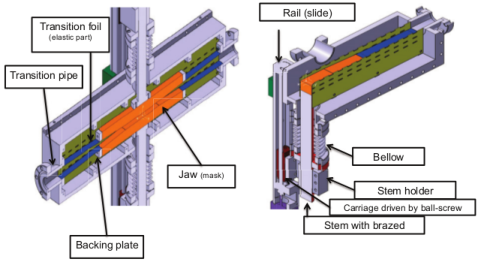
\includegraphics[width=0.8\textwidth]{ATF2_beamhalo_collimator.pdf}
\caption[Drawing of the beam halo collimator]{A drawing of the vertical beam halo collimator built into ATF2.\cite{NuriaCollimator2015}}
\label{fig:collimator}
\end{figure}

The two jaws can be moved individually to an arbitrary position, so that the edge of the jaw has a distance of between 2.6 and \SI{12}{\milli\metre} with respect to the centre. Therefore, the full aperture of the collimator structure can be between 5.2 and \SI{24}{\milli\metre}. The error on the position of the jaws is about \SI{0.04}{\milli\metre}.\\
As every component in a beam line, especially for such small beam sizes, is affecting the electromagnetic field of the passing beam, the collimator is designed to minimize the effect of inducing large wakefield. The concern of wakefields induced by the collimator is addressed in \cite{NuriaCollimator2015}. This thesis chapter focusses exclusively on the effect on the background level.

\begin{figure}
\centering
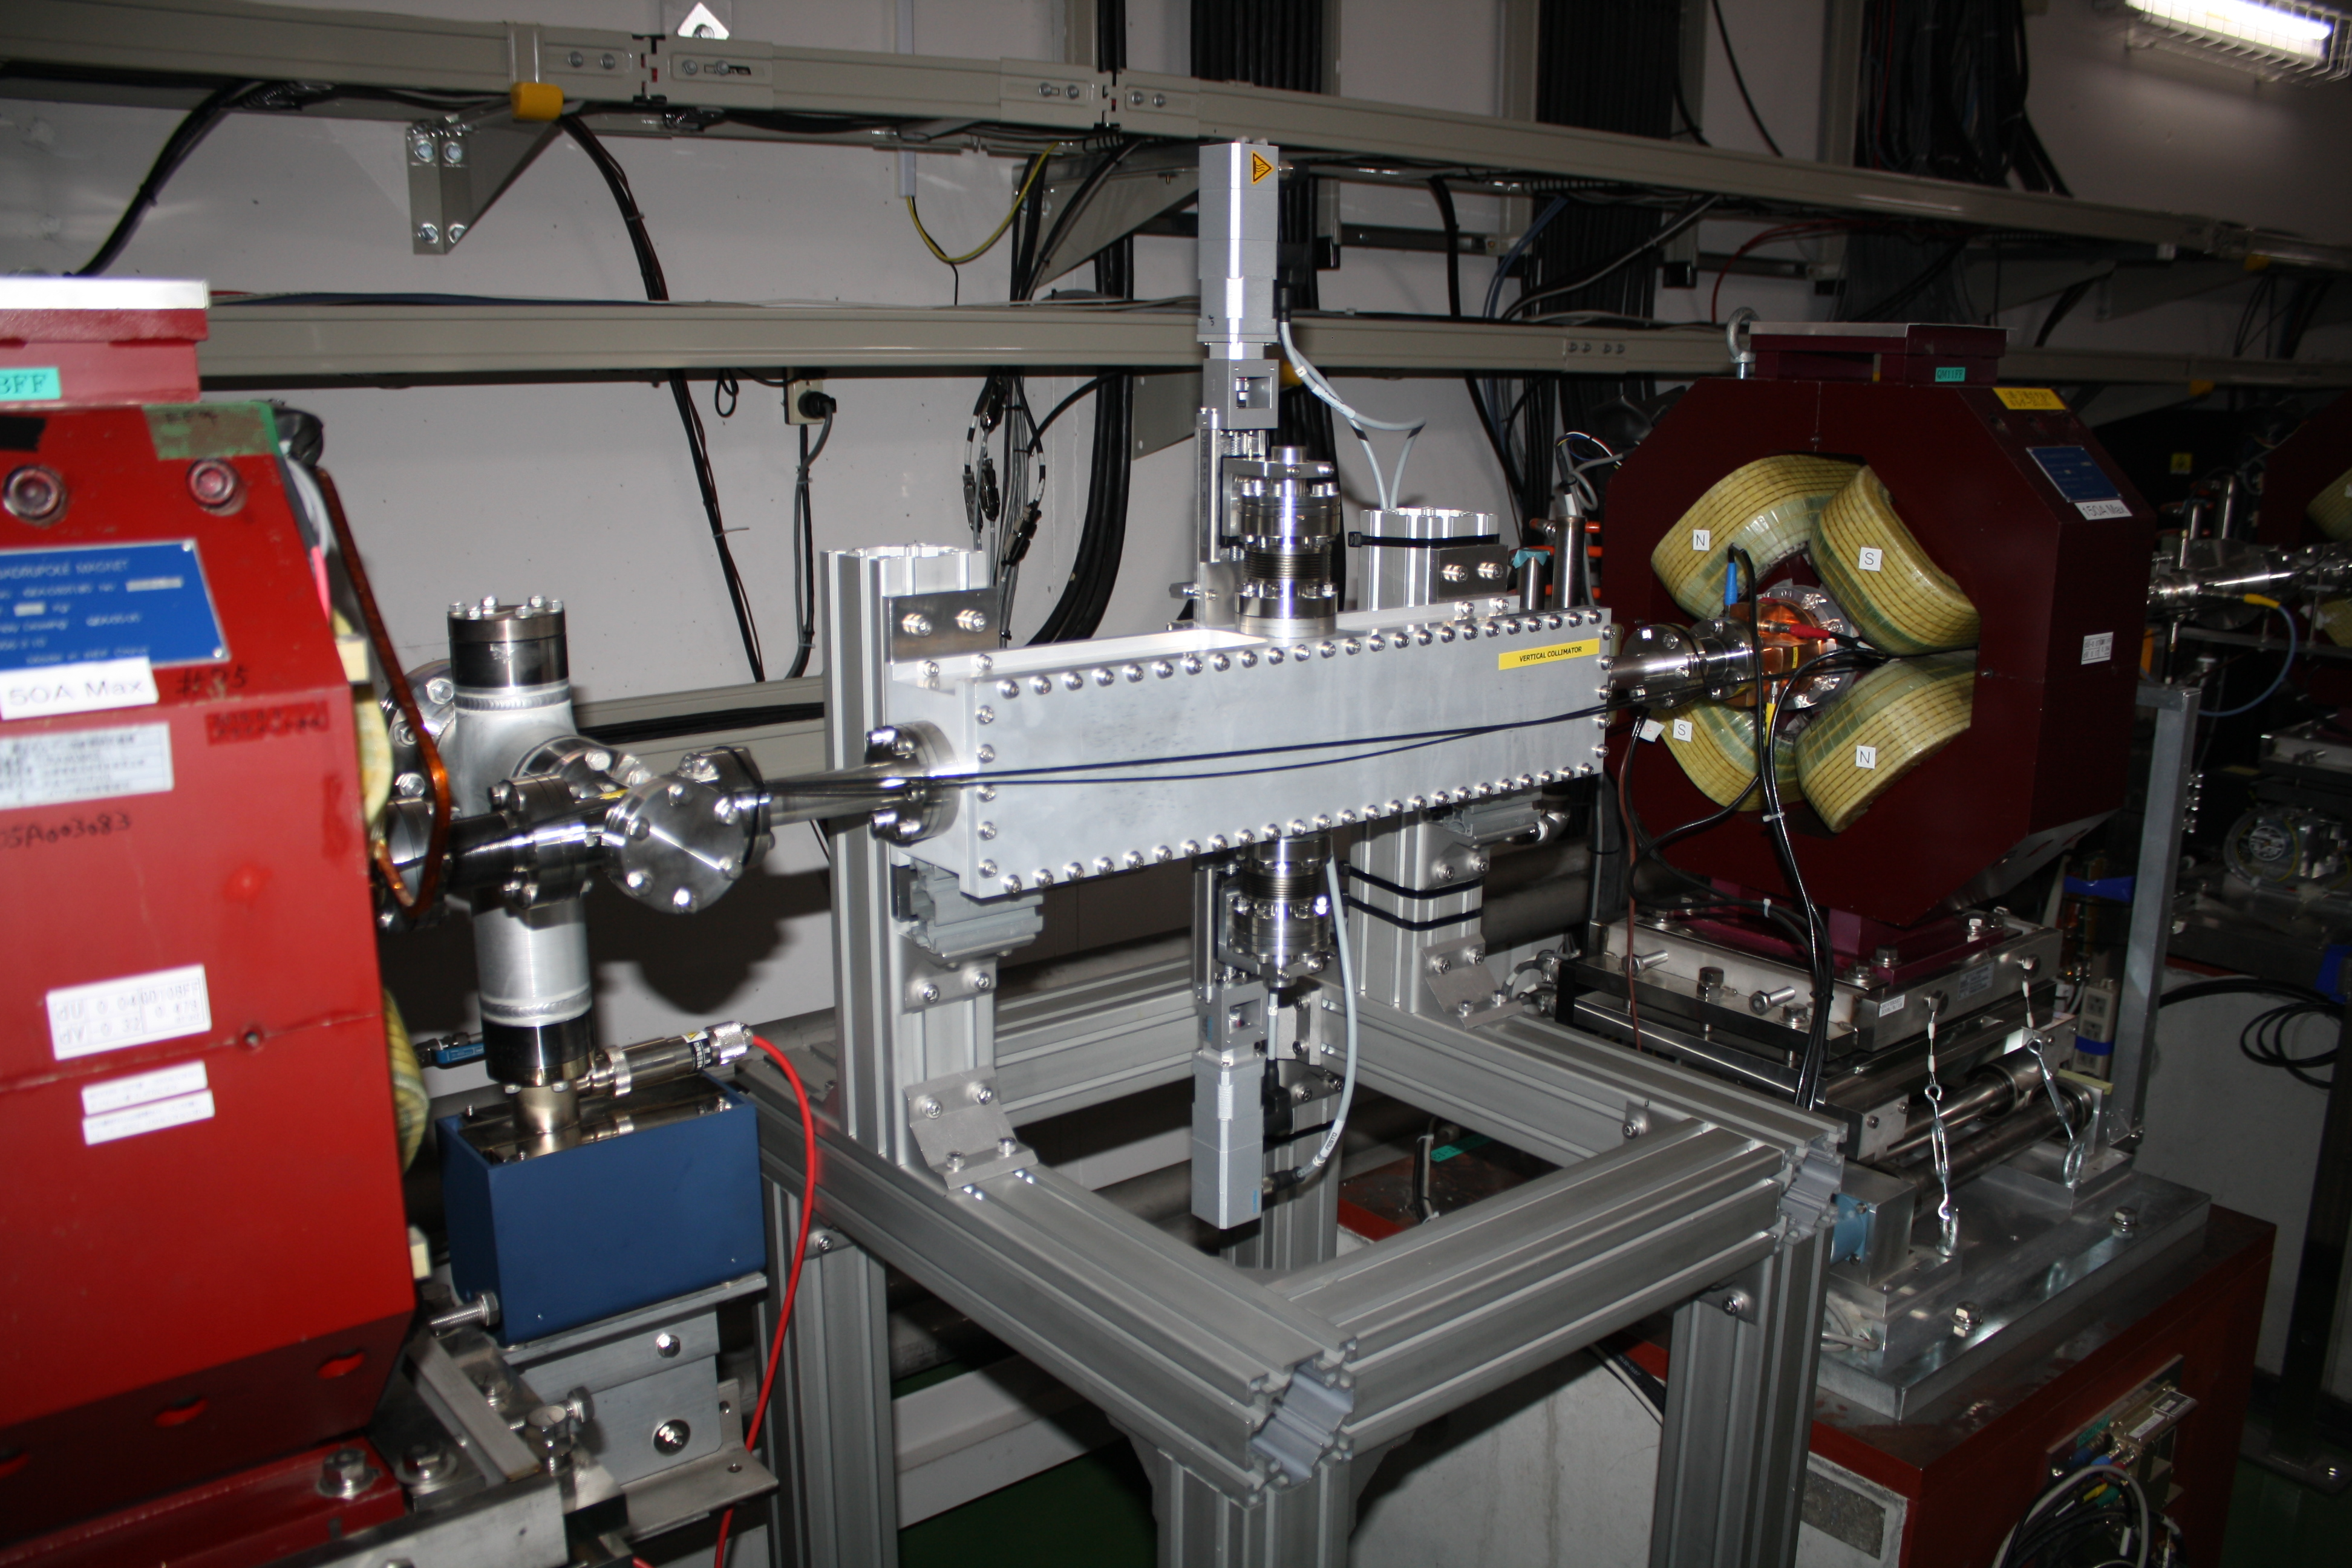
\includegraphics[width=0.8\textwidth]{Installed_Collimator.jpg}
\caption[Picture of the installed beam halo collimator]{A picture of the vertical beam halo collimator built into ATF2. The collimator jaws are within the evacuated structure. At the top and bottom of the structure, you can see the mover system for the two jaws.}
\label{fig:installed_collimator}
\end{figure}

\subsection{The Accelerator Test Facility 2}
\label{ATF2}

The Accelerator Test Facility 2 (ATF2) is an extension to the accelerator facility ATF at the research centre KEK in Japan. As can be seen in Figure~\ref{fig:ATF}, ATF consists of a linear accelerator which pre-accelerates the particles before they are accessing the dumping ring. Before the ATF2 was built, the beams were dumped after leaving the dumping ring through the short extraction line.\\ATF2 is a test bench for the FF system of the ILC and has two main goals: Focussing the low-emittance beam to \SI{37}{\nano\metre} in the vertical plane, and demonstrating the stability of the nanometre sized beam at the interaction point. So far a repeatable beam size of \SI{40}{\nano\metre} has been shown. Although the beam size goal of ATF2 seems to be too large compared to the ILC goal of \SI{9}{\nano\metre}, the ATF2 system is very close to the ILC FF. The beam size goal has to be scaled up for different lattice and beam conditions.

\begin{figure}
\centering
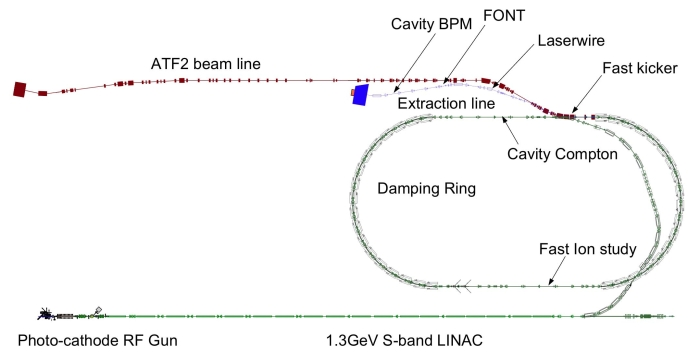
\includegraphics[width=0.6\textwidth]{ATF.jpg}
\caption[ATF accelerator]{A schematic of the ATF accelerator with the ATF2 extension. The ATF consists of a linear accelerator, a beam dump, the old extraction line, and the new ATF2 extension.}%TODO: cite the source of the ATF figure!
\label{fig:ATF}
\end{figure}

The vertical beam halo collimator and the Cherenkov detector, with which the background level in dependency of the collimator aperture was measured, are both located in the Final-Focus region of ATF2. The location of the collimator was chosen in such a way that the phase of the beta function is the same as at the IP. Due to that the effect of the collimation of the beam halo is then visible at the IP as desired. A schematic of the ATF2 lattice with the beam halo collimator and the Cherenkov detector is shown in Figure~\ref{fig:ATF2}. The Cherenkov detector was built and setup by a group of the Royal Holloway University of London (RHUL) because of which the detector is in the following referred to as the 'RHUL Cherenkov detector'. A more detailed description of this detector is given in Section~\ref{RHUL}.

\begin{figure}
\centering
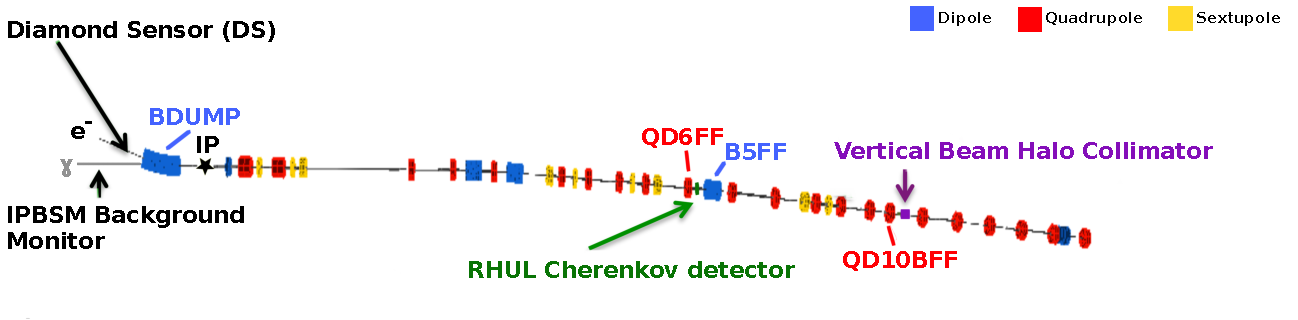
\includegraphics[width=\textwidth]{ATF2schematic.pdf}
\caption[ATF2]{A schematic of the ATF2 lattice. The beam direction is from right to left. The different magnets of the lattice are colour schemed: the bending dipole magnets are coloured in blue, the quadrupoles in red, and the sextupoles in yellow. The beam halo collimator is located before the quadrupole magnet 'QD10BFF', and the Cherenkov detector downstream between the dipole magnet 'B5FF' and the quadrupole magnet 'QD6FF'. After the interaction point (IP), the electron beam is bend in the last dipole magnet 'BDUMP' towards the beam dump. The neutral particles, like the photons, are continuing in a straight line where they can be monitored by the IPBSM Background Monitor. The Diamond Sensor (DS) can measure the shape of the beam core and the halo, before the beam is dumped.}
\label{fig:ATF2}
\end{figure}

\subsection{BDSIM}
\label{BDSIM}
\bdsim is a \geant extension toolkit for simulation of particle transport in accelerator beamlines. It was developed and is still supported by RHUL.
The geometry of lattice parts are described in classes within the \bdsim framework. Lattices, like the ATF2 lattice, can easily be built up by the pre-defined components. A figure of the ATF2 lattice visualized with the \bdsim software is shown in Figure~\ref{fig:ATF2_BDSIM}.
\begin{figure}
\centering
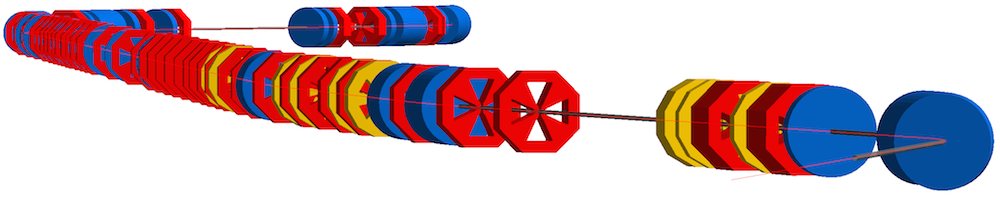
\includegraphics[width=0.7\textwidth]{atf_bdsim.png} %TODO: exchange with a recent one of ATF2
\caption[ATF2 lattice in \bdsim]{A part of the ATF2 lattice visualized with the \geant toolkit \bdsim.}
\label{fig:ATF2_BDSIM}
\end{figure}
Accelerator descriptions from other tools such as MADX can be converted to \bdsim input. 
%---------------------------------------------------
\subsection{Background studies}
\subsubsection{RHUL Cherenkov detector}
\label{RHUL}

The RHUL Cherenkov detector was built by a group from the Royal Holloway University of London. It uses the Hamamatsu PMT, which was used for a laserwire sensor that was located at the same position before. The Cherenkov detector itself is using aerogel\footnote{SP15, index 1.015, 4 slices, 4 cm$^2$, 5 cm deep}. A light pipe, with a profile area of \SI{10}{\centi\metre\square} and a total length of \SI{35}{\centi\metre}, directs the light from the aerogel to the PMT.

\begin{figure}
\centering
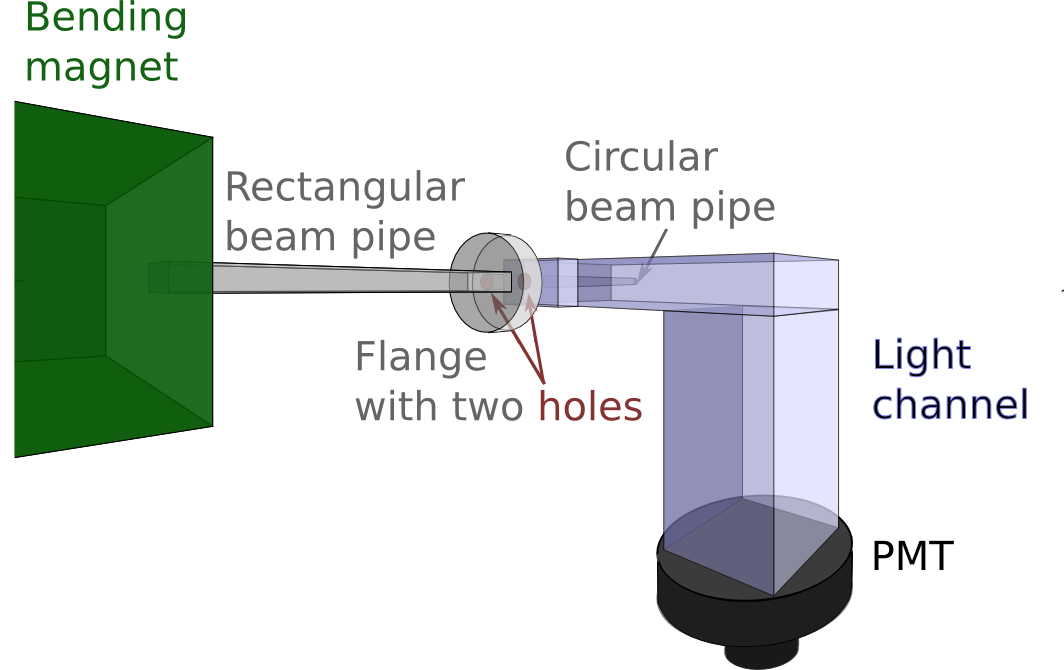
\includegraphics[width=0.8\textwidth]{drawing_CherenkovSetup.png}
\caption[Schematic drawing of the RHUL Cherenkov detector setup]{A perspective schematic of the RHUL Cherenkov detector setup in ATF2. The electrons of the beam core are bent in the dipole magnet, and continue through the rectangular and circular beam pipes along the ATF2 beam line. The neutral particles on the other hand, which are not deflected in the magnetic field, are continuing on a straight line through the rectangular beam pipe, and enter the RHUL Cherenkov detector through the second window in the flange. The light signals are collected by the PMT.}
\label{fig:RHUL_Cherenkov_Drawing}
\end{figure}

\begin{figure}
\begin{center}
\resizebox{.9\textwidth}{!}{%
\includegraphics[height=0.35\textheight]{CherenkovDetector_inBeamLine1.jpg}%
\quad
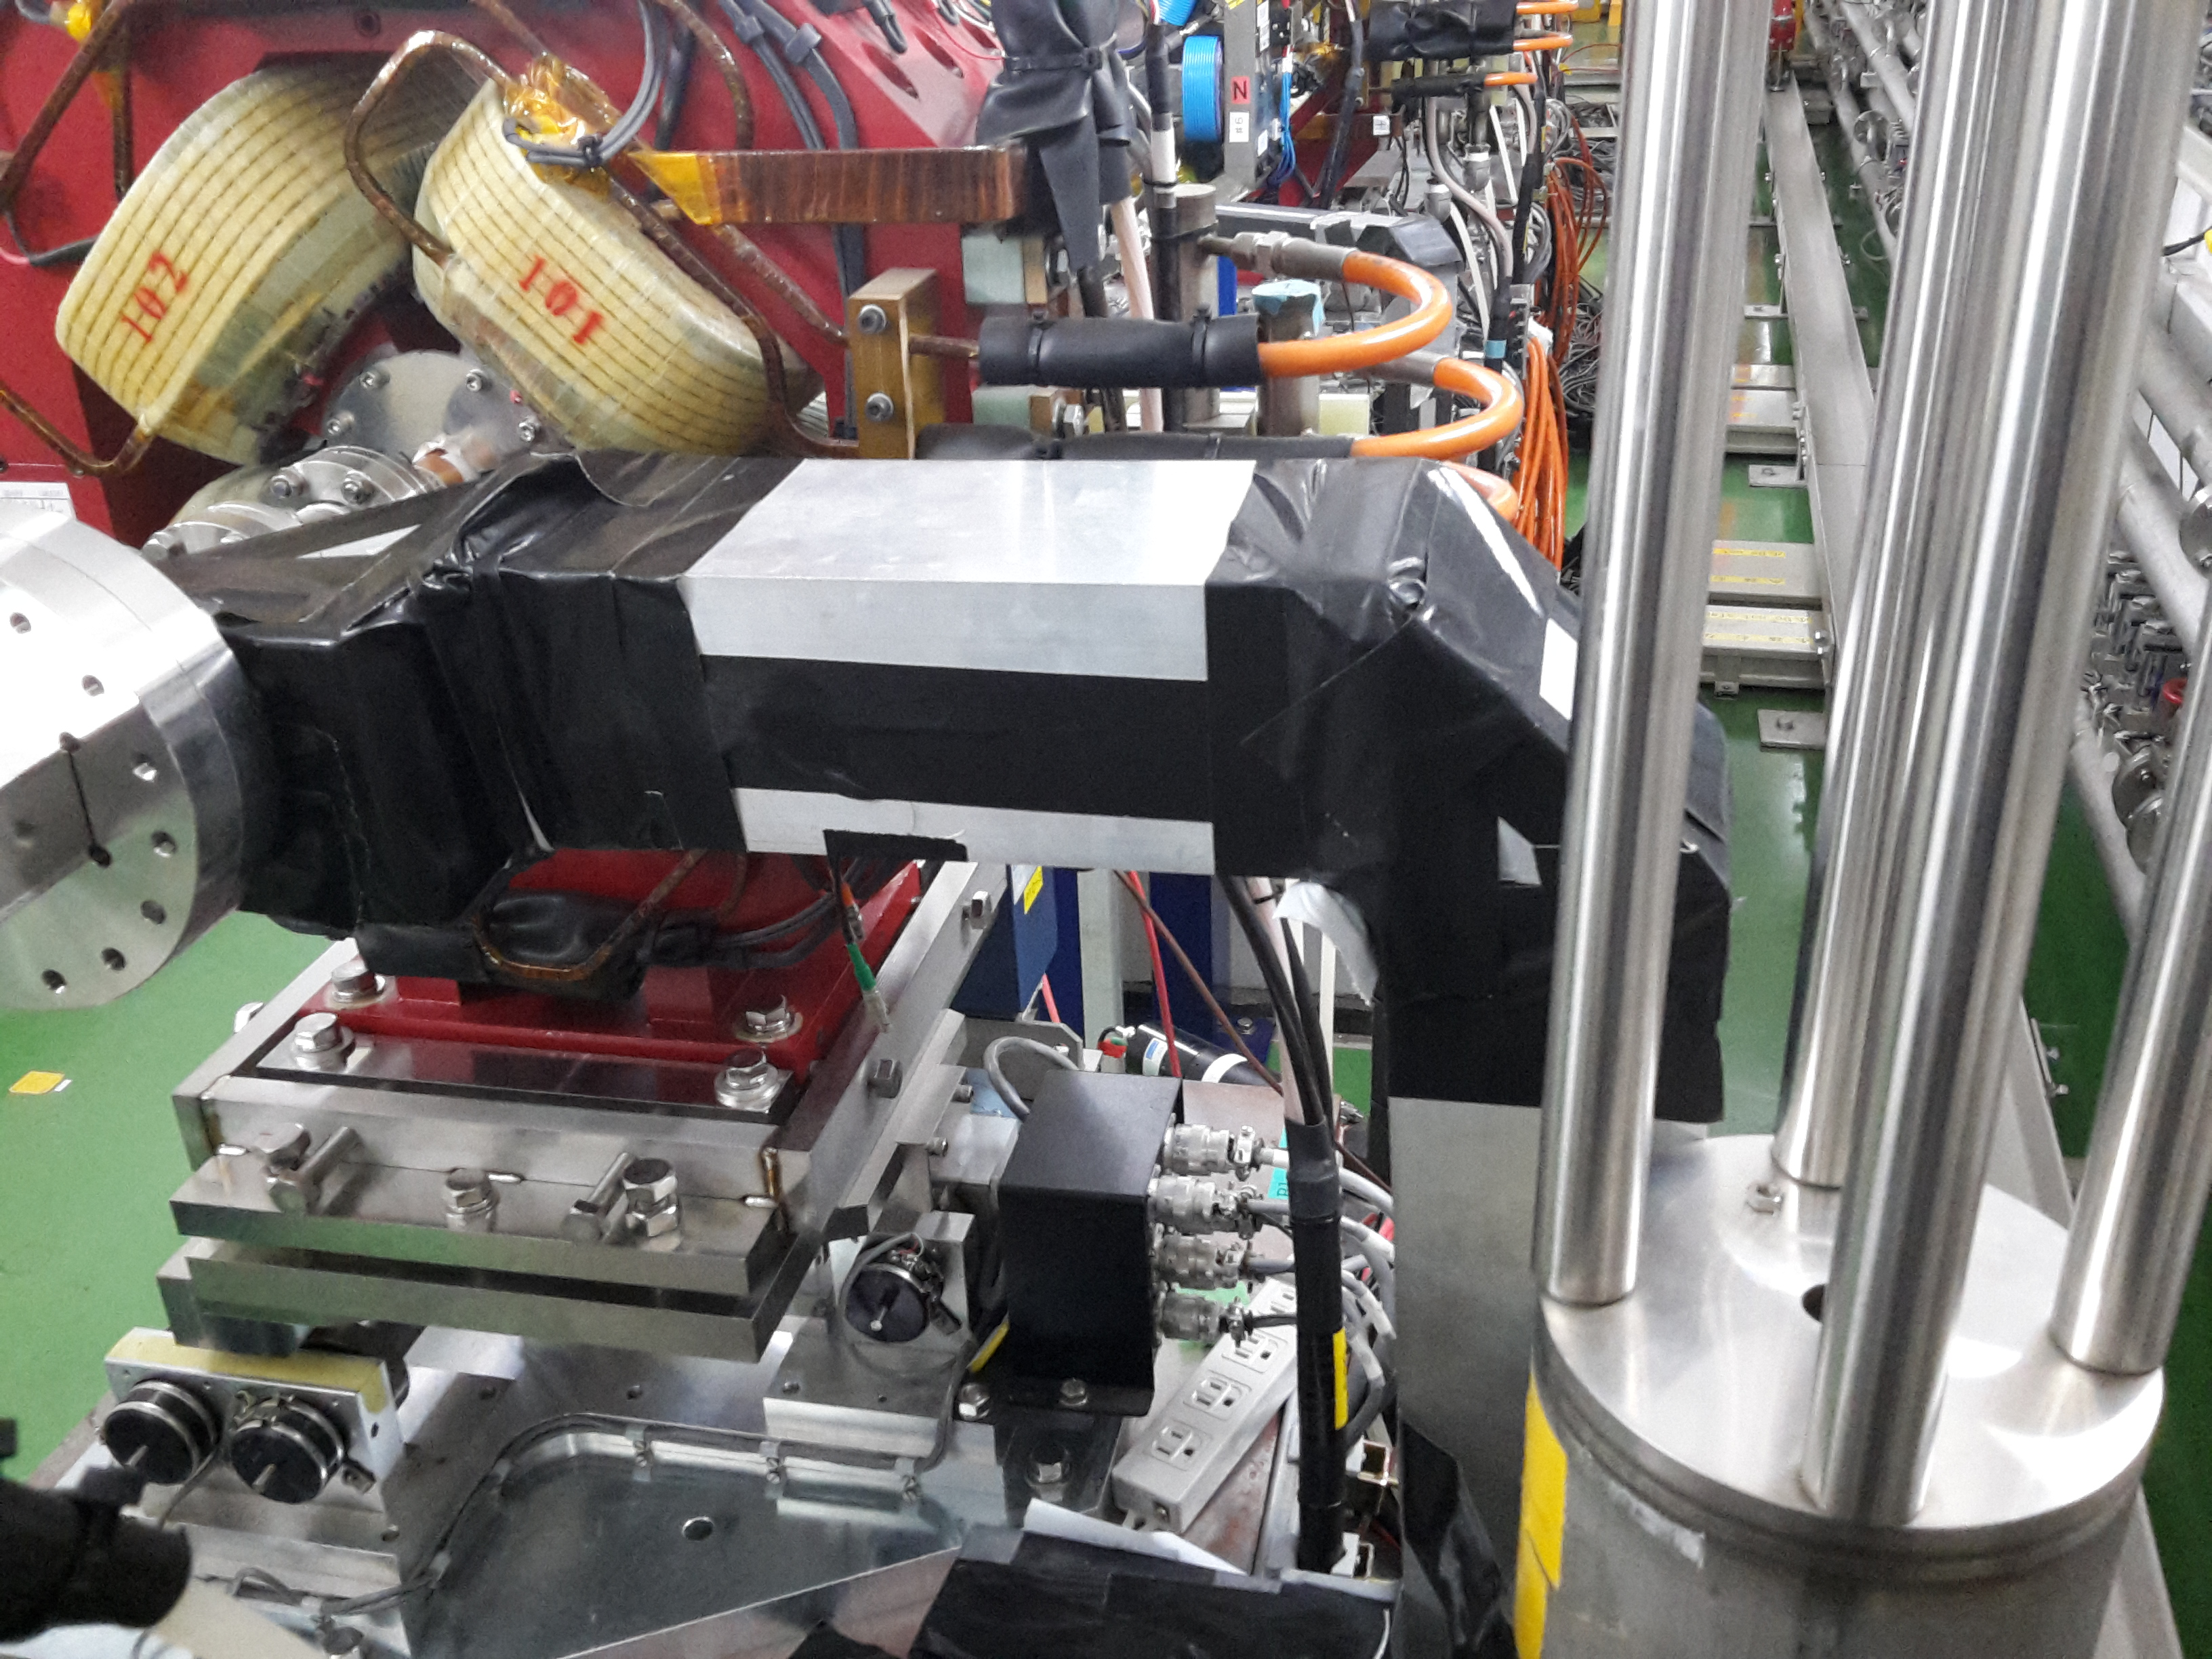
\includegraphics[height=0.35\textheight]{CherenkovDetector_inBeamLine2.jpg}%
}
\caption[Pictures of the RHUL Cherenkov detector]{Pictures of the RHUL Cherenkov detector in ATF2. The aerogel detector and the light channel is positioned behind a flange that connects a rectangular beam pipe with a circular one. The flange has two openings, one for the circular beam pipe, another one covered by a plastic window through which the photons leave the rectangular beam pipe and enter the RHUL Cherencov detector.}
\label{fig:RHUL_Cherenkov}
\end{center}
\end{figure}

\begin{figure}
\centering
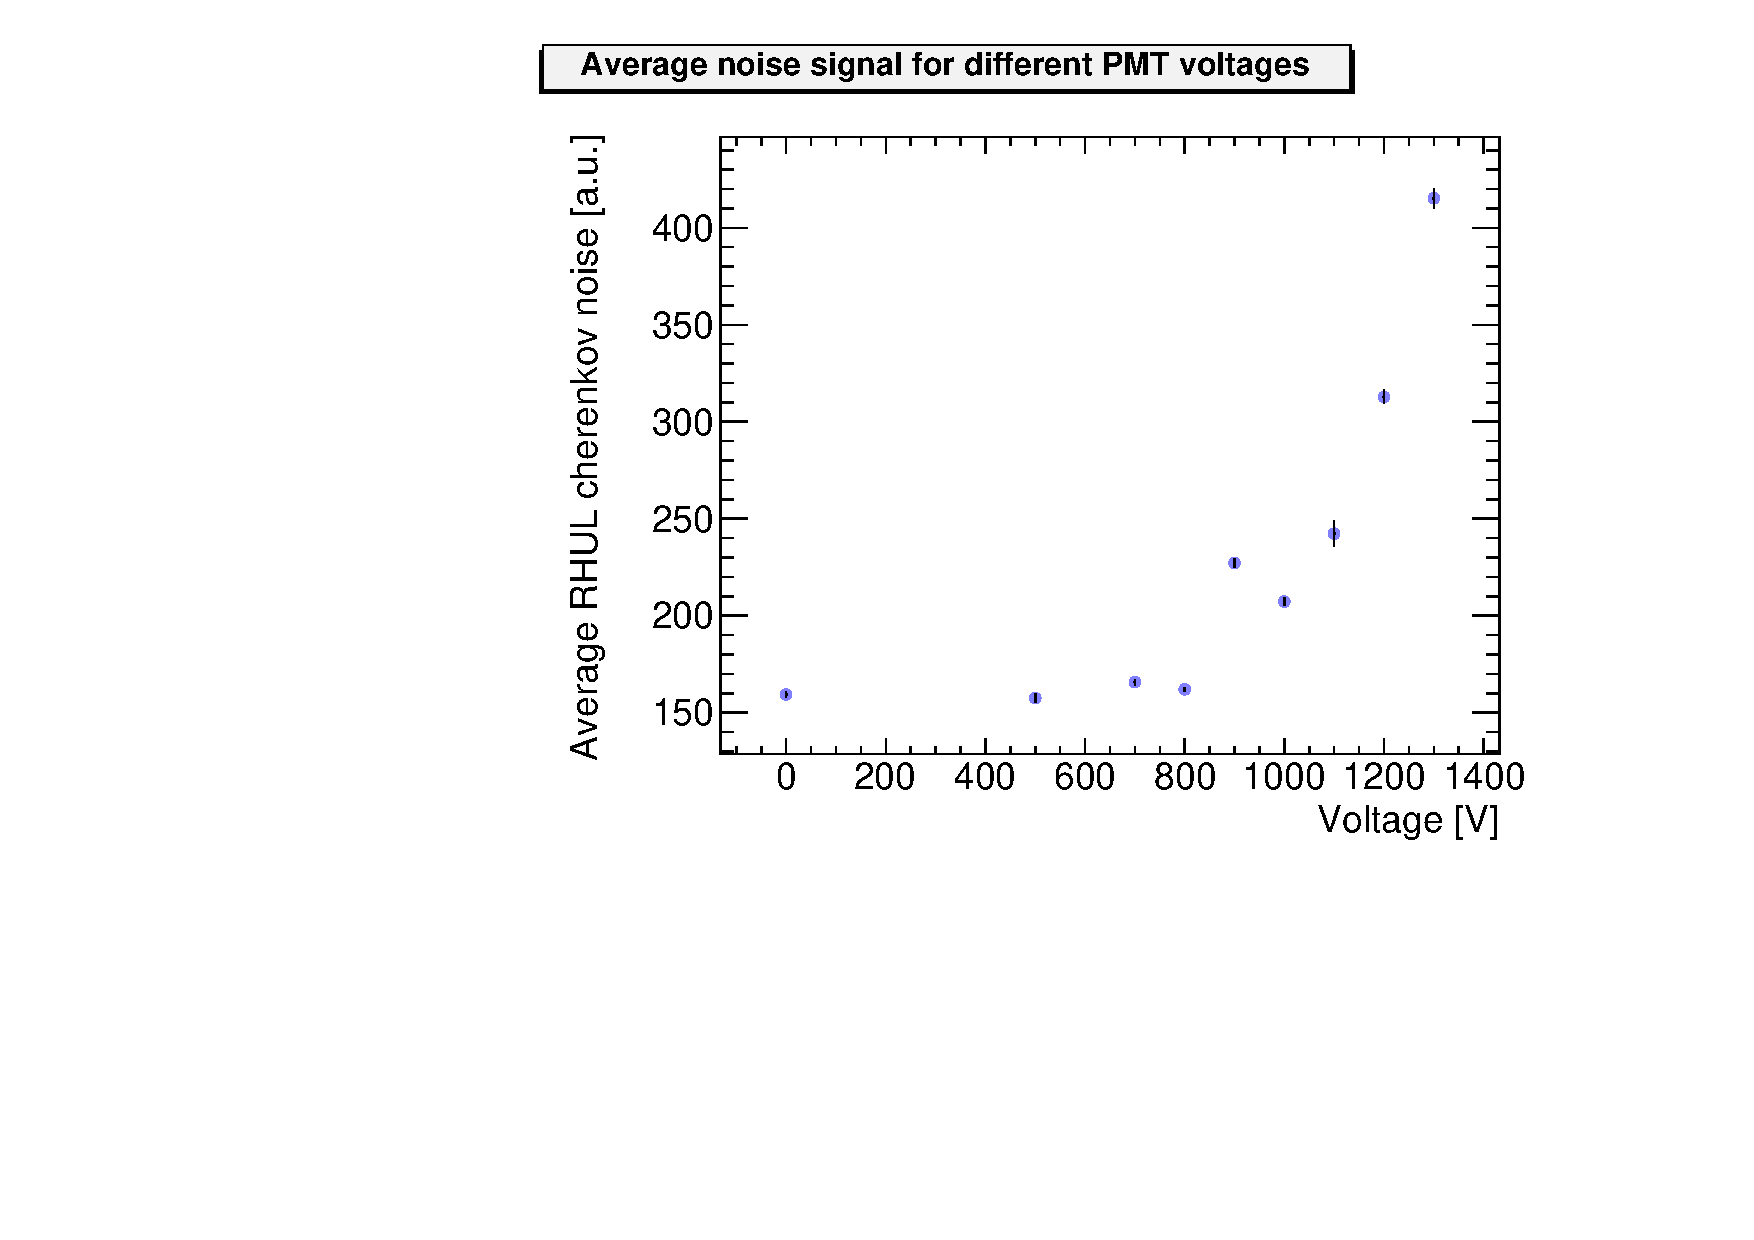
\includegraphics[width=\textwidth]{AverageNoise_perVoltage.pdf}
\caption[RHUL Cherenkov detector noise]{Average noise signal as a function of the voltage applied to the detector PMT. The noise was measured when the ATF beam was turned off. For each voltage, 500 or 1000 ADC pulses of noise were recorded, and the noise averaged over the number of pulses. The error bars to the mean values are the standard deviation of the mean.}
\label{fig:AverageNoise}
\end{figure}
Figure ~\ref{fig:AverageNoise} shows the mean values of the noise measurements for different PMT voltages. For every point either 500 or 1000 ADC pulses were recorded and averaged. The error bars represent the standard deviation on the mean value calculated by $SD=\frac{\sigma}{\sqrt{N}}$, where $\sigma$ is the RMS of the noise distribution at each point and N the number of pulses.\\
At around \SI{800}{\volt} the effect of dark current in the PMT starts getting prominent wherefore the noise rises exponentially. For the data shown in the following, the noise is already subtracted. As the data was taken only for these voltages, for which noise measurements were done, the mean value of noise is subtracted from every signal pulse appropriately. Therefore the rise in noise is automatically taken into account for higher voltages.

\subsubsection{Collimator apertures scan - for different intensities and vacuum pressures}
\label{aperture_scans}
Scans of the background for different collimator apertures were done, first for symmetric positions of the lower and upper jaw around the centre, later for asymmetric positions. Additionally, a scan was done with one jaw fully extracted and the other one moving to certain positions. The last scan is referred to as the 'half aperture scan', whereas the first two scans are the 'symmetric' and the 'asymmetric' scans.\\
Figure ~\ref{fig:AverageSignal_Aperture_BeamIntensities} shows the plot of the average detector signals for the asymmetric scan of different collimator apertures. The scans were done for five different beam intensities. It is clear that the background level rises with increase in intensity. The characteristic shape of the scan is however conserved: the background level is constant while closing the collimator from a full aperture of \SI{24}{\milli\metre} to about \SI{12}{\milli\metre}. When closing to \SI{10}{\milli\metre} the background level drops, and rises again when closing the collimator completely, i.e. to \SI{6}{\milli\metre} full aperture. This characteristic drop and rise between 12 and \SI{6}{\milli\metre} is on the one hand proof of the proper functionality of moving the collimator jaws, on the other hand leaves some questions open: where are the background particles originating that are cut away by the collimator, and does the rise in background mean that the collimator is showering the beam halo particles? Which qualities do these produced background particles have?\\
These questions are addressed in Chapter ~\ref{sec:BDSIM_sim}, in which the effect of the collimator is simulated in a BDSIM simulation.
\newline
Figure~\ref{fig:AverageSignal_Aperture_VacuumPressures} shows a plot of a measurement done in the same way but for two different vacuum pressures: \SI{4.9e-7}{\pascal} and \SI{1.06e-6}{\pascal}. The graphs are directly comparable as they both show data taken for a beam intensity of \num{0.5}$\pm$\num{0.03e10}. It is clear and as expected that the background level is higher for a worse vacuum, i.e. for a higher pressure. Nevertheless, the background level is not only shifted. By closing the collimator to an aperture of \SI{10}{\milli\metre}, the background reduced to almost the same level whereas at the plateau (between 12 and \SI{24}{\milli\metre}) the background level for the smaller pressure is almost double. The collimator reduces therefore the background dramatically, especially at high background rates.

\begin{figure}
\centering
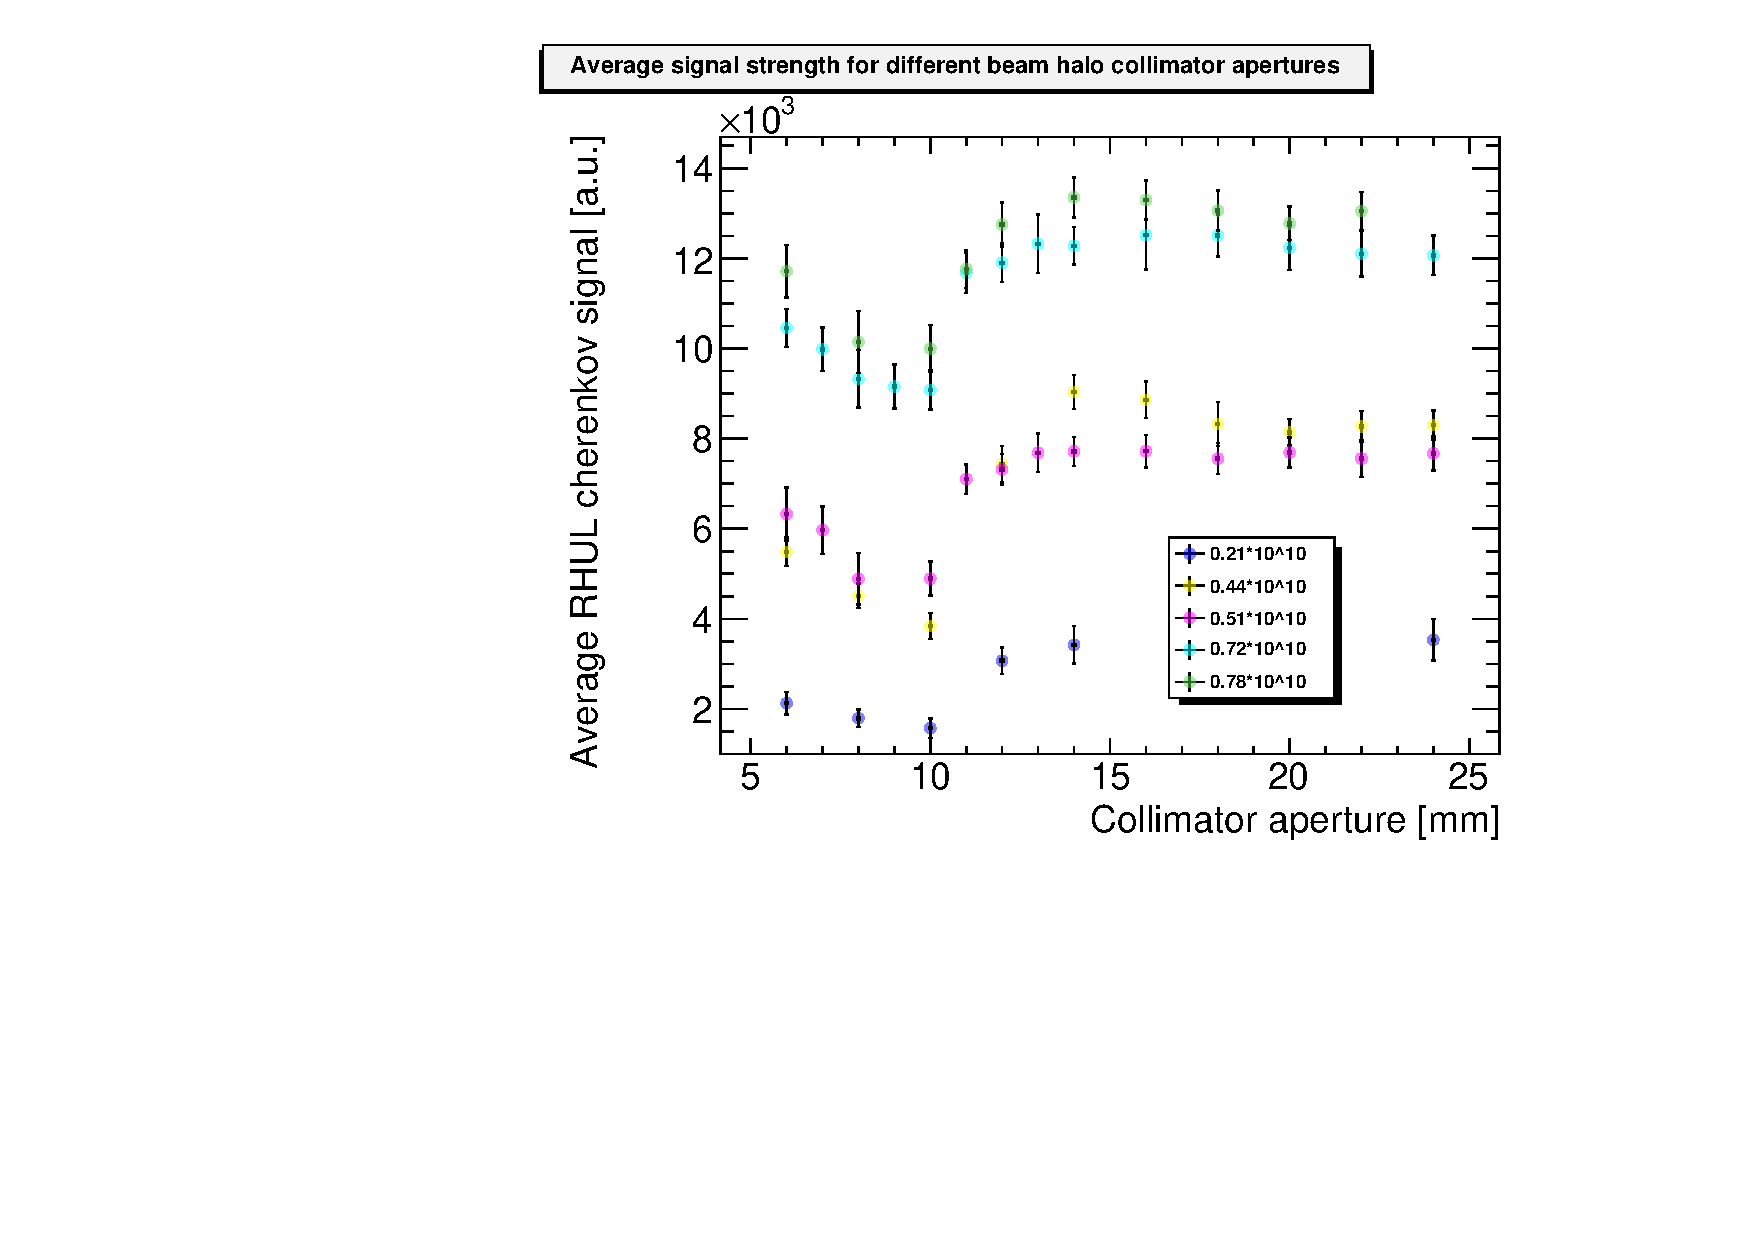
\includegraphics[width=\textwidth]{AverageSignal_perAperture.pdf}
\caption[RHUL Cherenkov detector signal vs. collimator aperture: different beam intensities]{Average signal as a function of the full aperture of the vertical beam halo collimator. The signal was measured for different beam intensities [\num{10e10}]: 0.21$\pm$0.02, 0.44$\pm$0.02, 0.51$\pm$0.02, 0.72$\pm$0.02 and 0.78$\pm$0.02, while the PMT voltage was constant at \SI{900}{\volt}. For each aperture, 500 ADC pulses were recorded, and the signal was averaged over the number of pulses. The error bars to the mean values are the standard deviation of the signal distributions at each point.\\For some scans, the data was not taken for all apertures. Therefore, especially the graph for the beam intensity of \num{0.21}$\pm$\num{0.02e10} is missing data points for the half millimetre steps and between 14 and \SI{24}{\milli\metre}.}
\label{fig:AverageSignal_Aperture_BeamIntensities}
\end{figure}
\begin{figure}
\centering
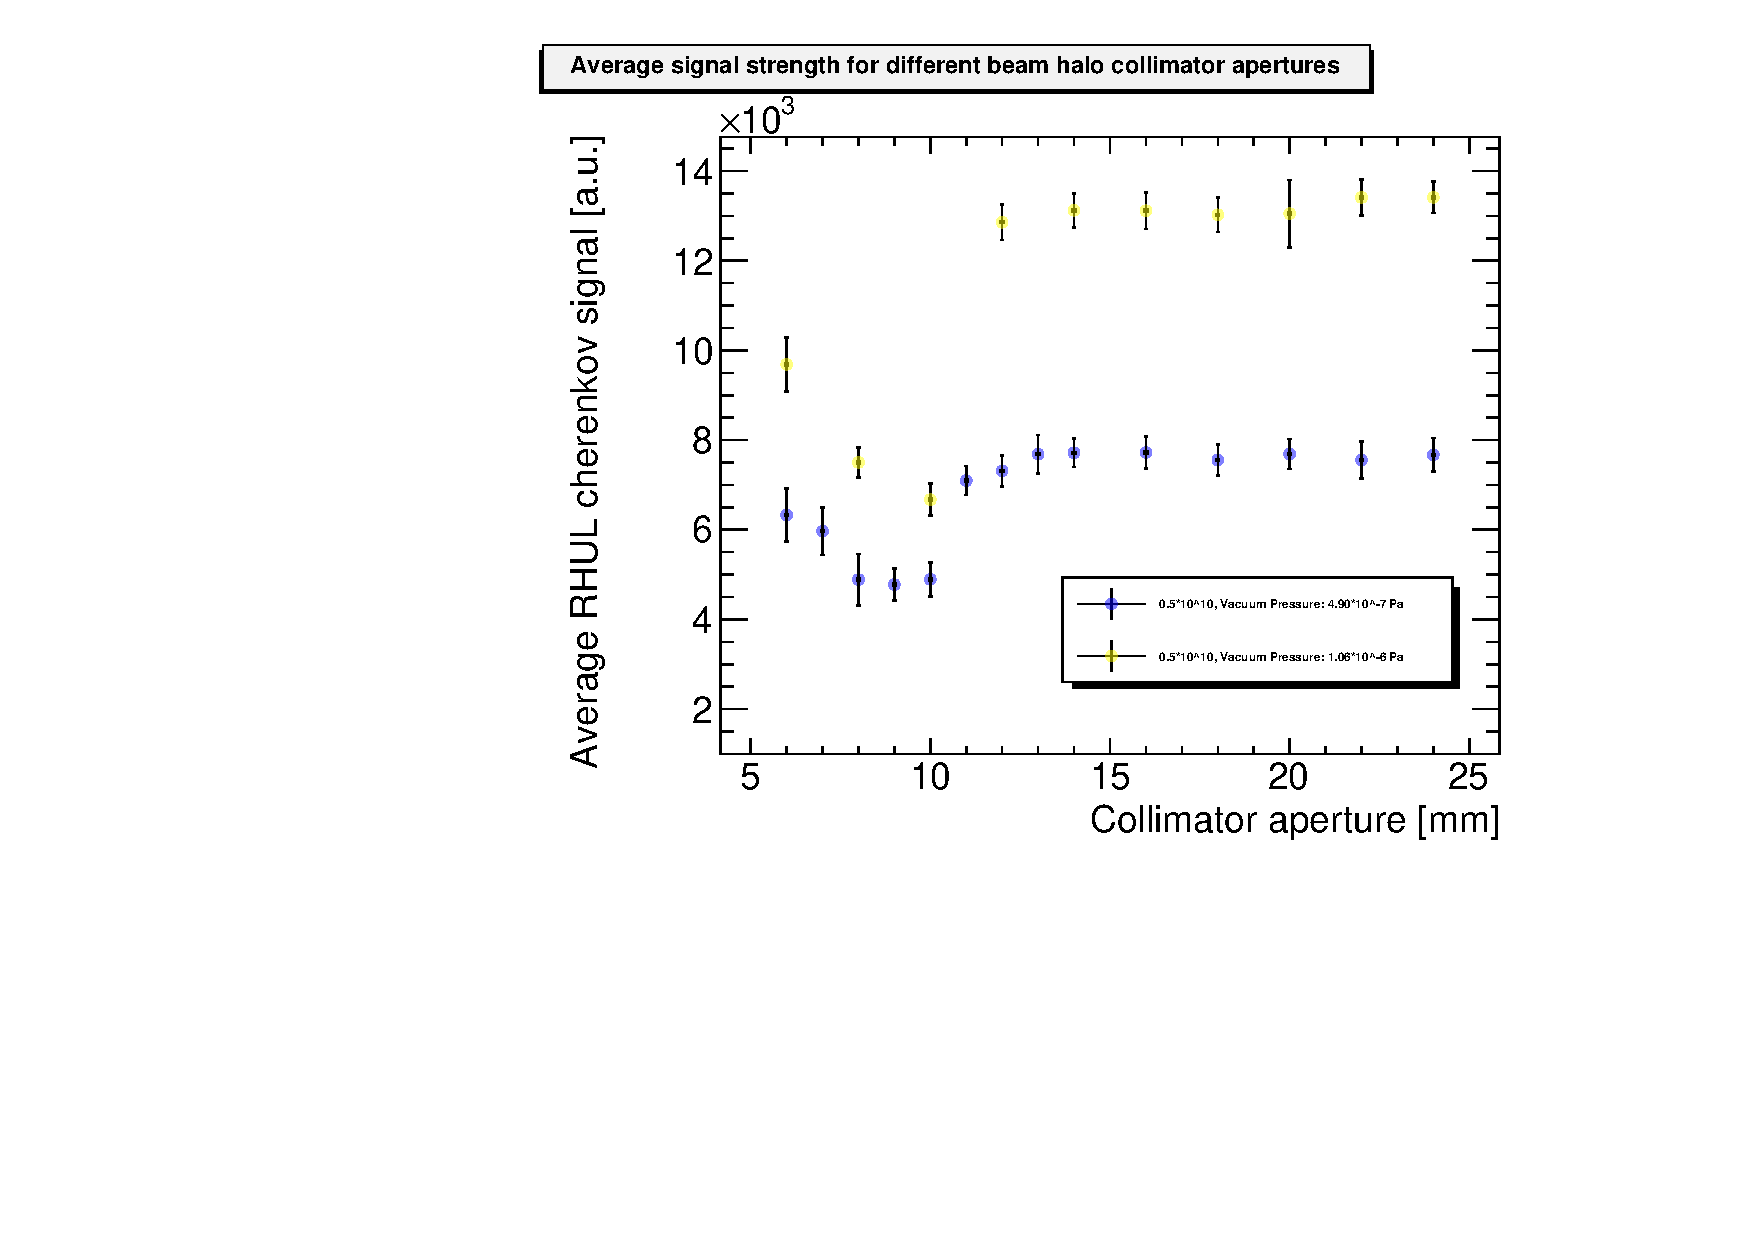
\includegraphics[width=\textwidth]{AverageSignal_perAperture_VacuumPressures.pdf}
\caption[RHUL Cherenkov detector signal vs. collimator aperture: different vacuum pressures]{Average signal as a function of the full aperture of the vertical beam halo collimator. The signal was measured for a beam intensity of \num{0.5}$\pm$\num{0.03e10} and a PMT voltage of \SI{900}{\volt}. The vacuum pressure was lowered from \SI{4.9e-7}{\pascal} to \SI{1.06e-6}{\pascal}. For each aperture, 500 ADC pulses were recorded, and the signal was averaged over the number of pulses. The error bars to the mean values are the standard deviation of the signal distributions at each point.}
\label{fig:AverageSignal_Aperture_VacuumPressures}
\end{figure}

\subsubsection{Test of the collimator alignment with respect to the beam position}
\label{collimator_alignment}
The next measurement sets are done to experimentally test whether the collimator is aligned in such a way that the beam is going through the centre between the jaws. The idea is that the background signal should be asymmetric if the beam is closer to one or the other side.\\Figure~\ref{fig:AverageSignal_HalfAperture} shows a plot of a measurement where one of the jaws was moved while the other jaw stayed in the fully extracted position. It is clear that moving the upper jaw shows the same characteristic background shape as before in the plots~\ref{fig:AverageSignal_Aperture_BeamIntensities} and \ref{fig:AverageSignal_Aperture_VacuumPressures}. But moving the lower jaw only shows no significant change in background. This leaves one with the possible conclusion that the beam is not in the centre between the two jaws but rather closer to the upper jaw. One could then say that also the background shape of the previous plots are only influenced by the upper jaw only. To confirm this conclusion, more measurements of this kind should be done to exclude a statistical fluctuation or simply a mistake in the process of data taking.
\newline
The next four figures show scans with asymmetric jaw positions around a certain value, i.e. 4 or \SI{5}{\milli\metre}. For each value, around which the jaws were moved, two measurements were done for the intensities of \num{0.84}$\pm$\num{0.03e10} and \num{1.01}$\pm$\num{0.03e10}. The plots are showing the background level in dependency of the position of the upper and lower jaw. As one jaw was moved in, the other one was simultaneously moved out, because of which the data line is diagonal in the diagrams. In all of the plots the drop in background level is clearly visible for a upper jaw position of \SI{5}{\milli\metre}, which follows the same behaviour as before. By closing the jaw more, the background level rises again and peaks for the minimal upper jaw position as the collimator jaw moves into the beam. All this seems to be consistent with the assumption that also here the lower jaw doesn't effect the beam in any way. Otherwise the plot would also show low background intensities for lower jaw positions of below \SI{5}{\milli\metre} which is not the case.\\
Especially significant is Figure~\ref{fig:AverageSignal_Asymmetric_5mm_101} with an identical background behaviour as in the measurements in Section~\ref{aperture_scans}. Also here it would be easier to make meaningful statements if the measurements would have more data points for larger jaw position regions, especially for the same positions in all plots.
\begin{figure}
\centering
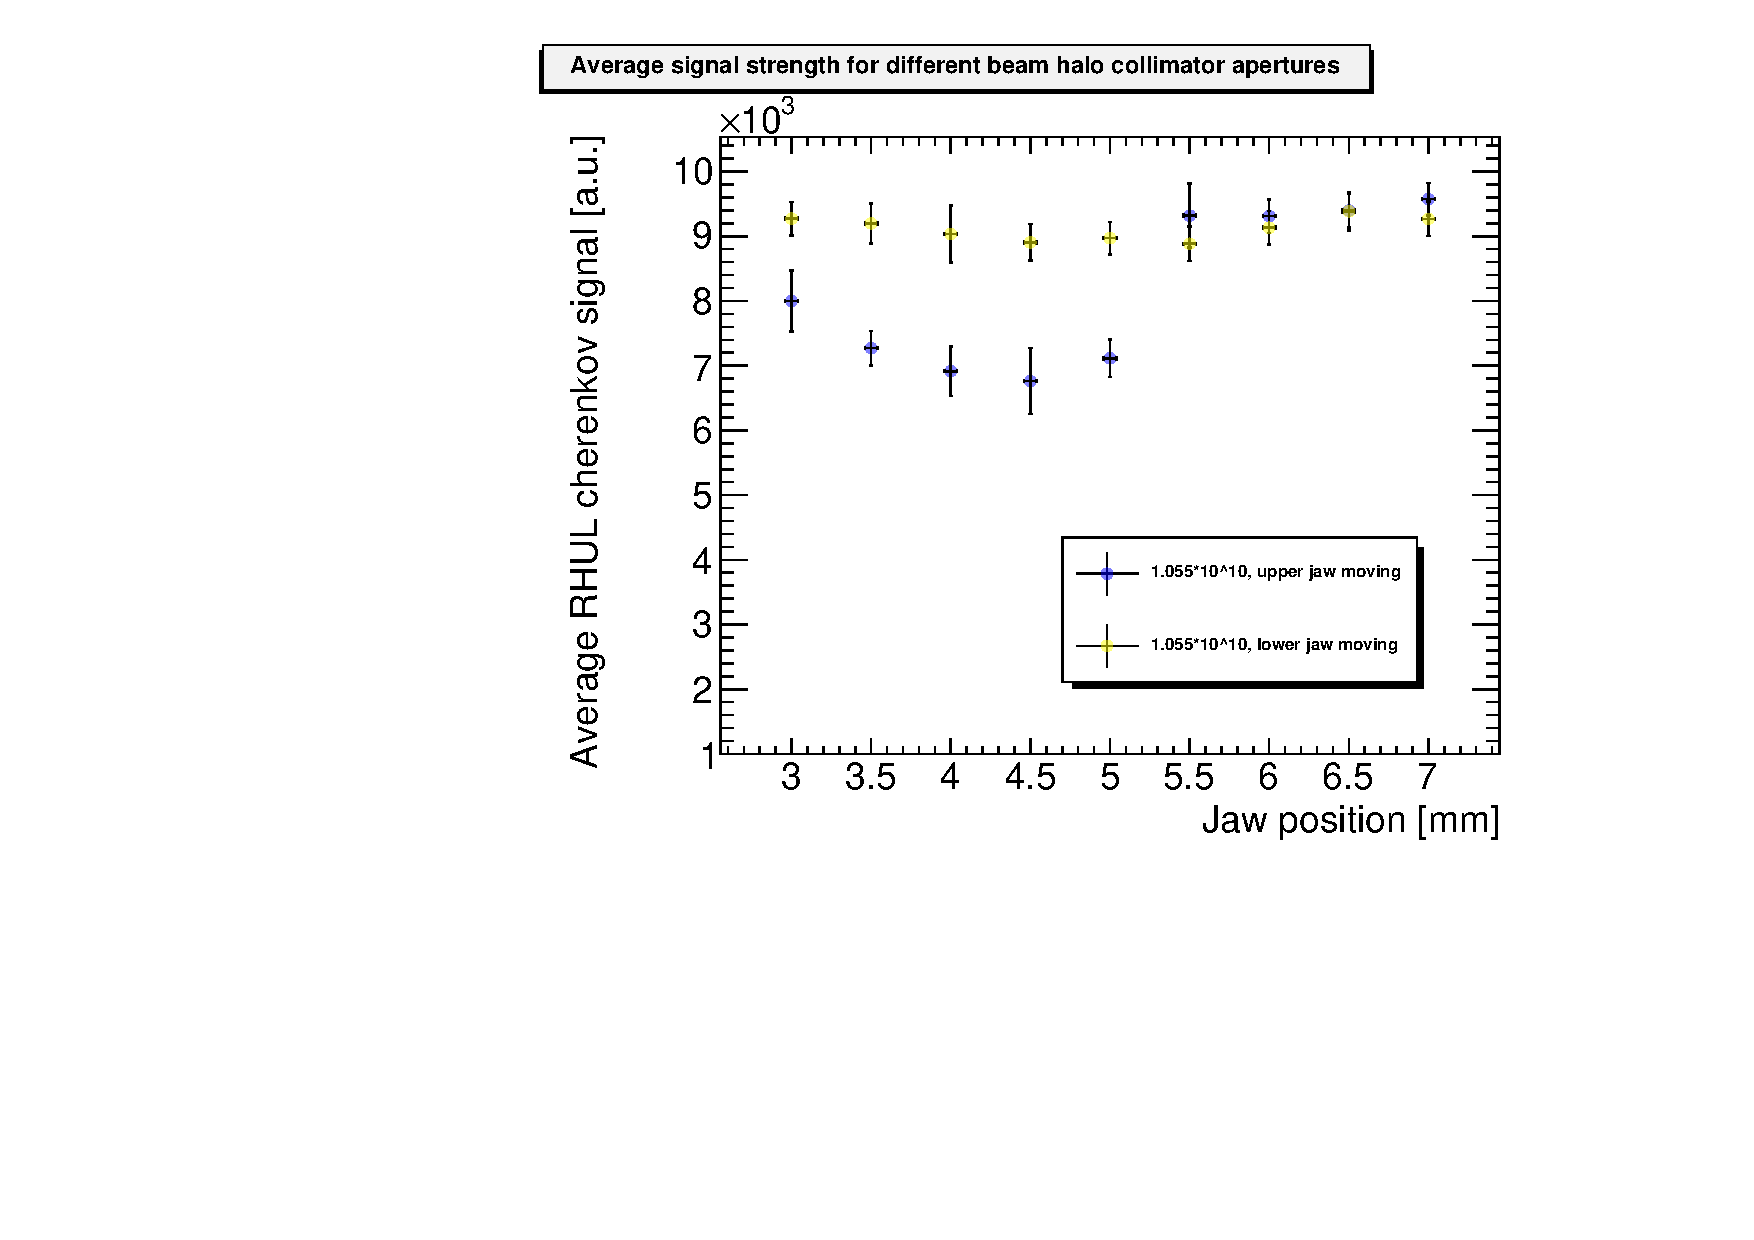
\includegraphics[width=\textwidth]{AverageSignal_perJawPosition.pdf}
\caption[RHUL Cherenkov detector signal vs. collimator half aperture]{Average signal as a function of the position of the upper/lower jaw of the vertical beam halo collimator. The signal was measured for a beam intensity of \num{1.05}$\pm$\num{0.04e10} and a PMT voltage of \SI{800}{\volt}. First, the lower jaw was fixed to its open position (\SI{12}{\milli\metre}) and the upper jaw was moved to the positions plotted, then vice versa. For each jaw position, 500 ADC pulses were recorded, and the signal was averaged over the number of pulses. The error bars to the mean values are the standard deviation of the signal distributions at each point.}
\label{fig:AverageSignal_HalfAperture}
\end{figure}
\begin{figure}
\begin{subfigure}[b]{0.5\textwidth}
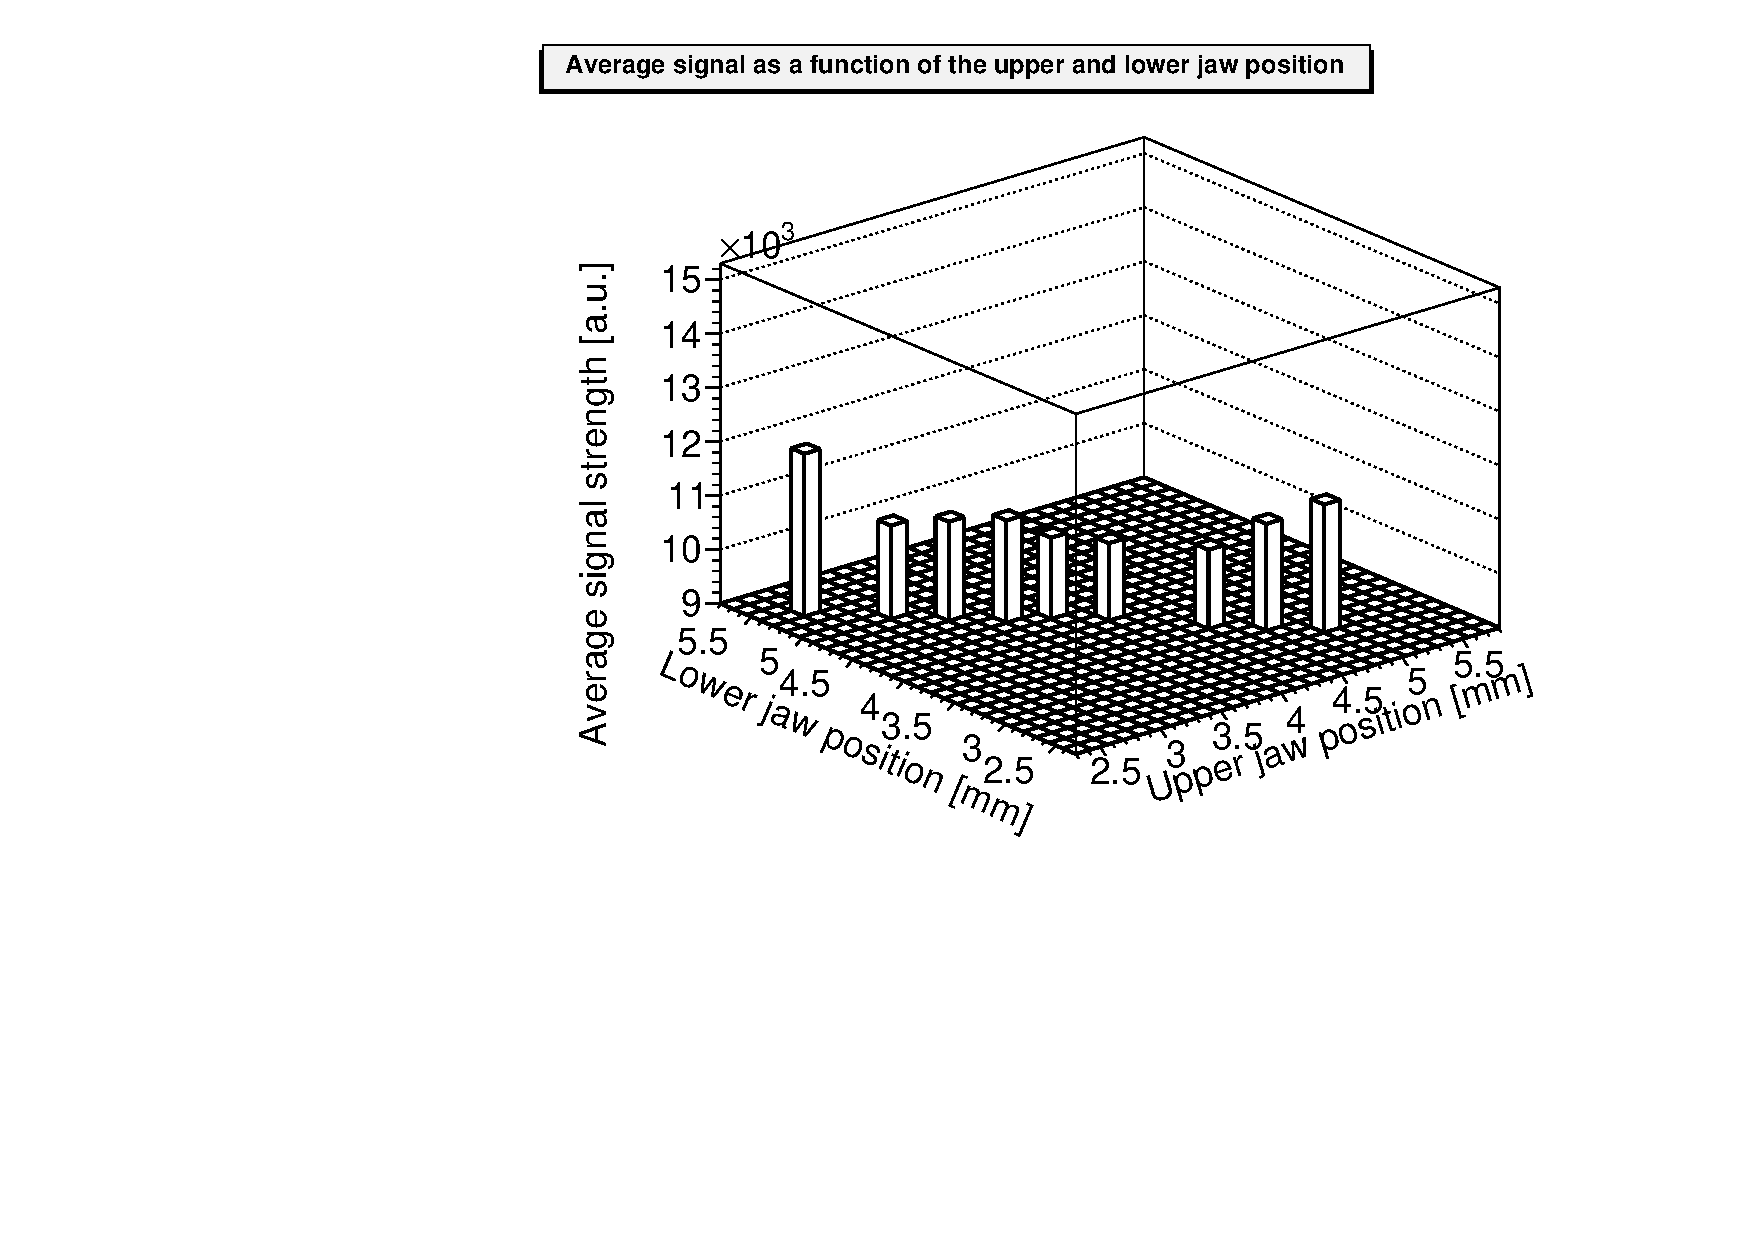
\includegraphics[width=\textwidth]{AsymmetricScan_4mm_beamintensity084_lego.pdf}
\end{subfigure}
\begin{subfigure}[b]{0.5\textwidth}
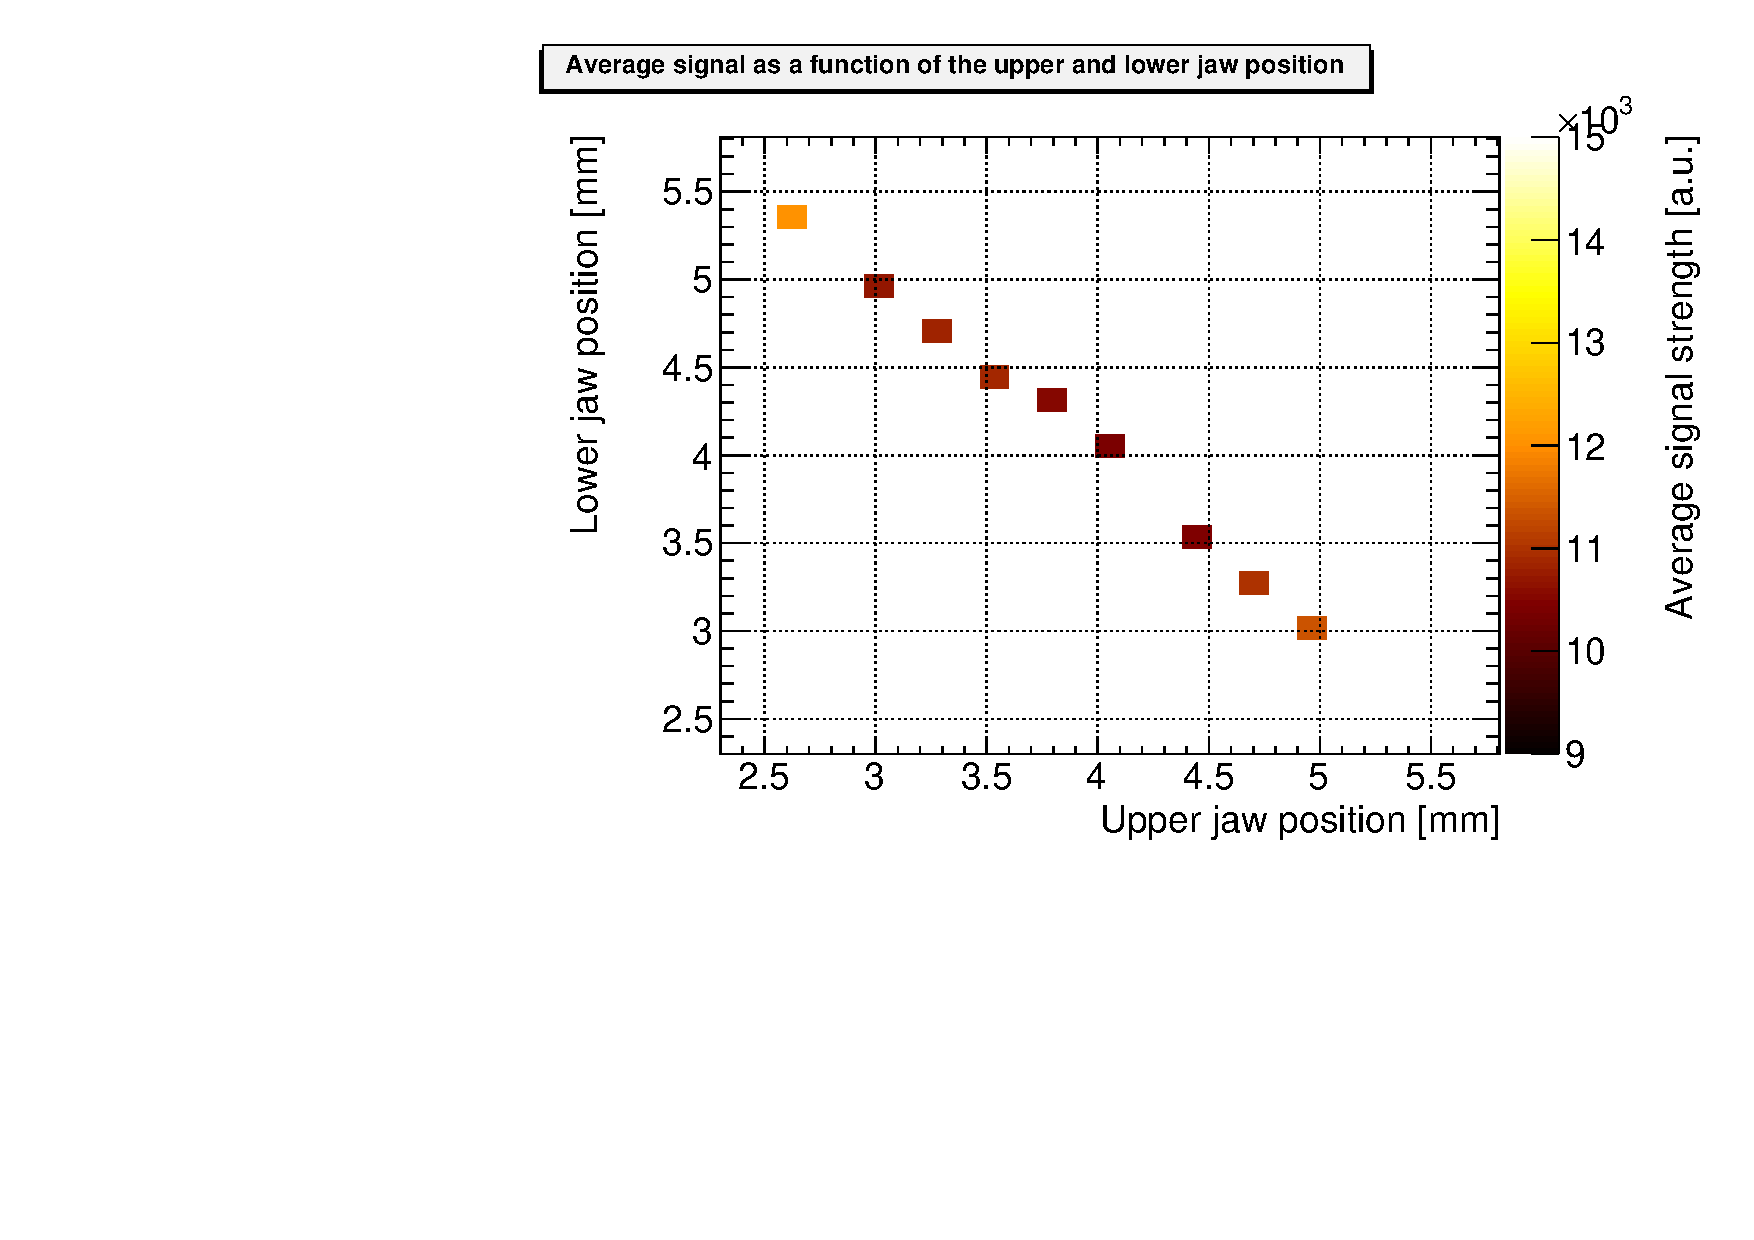
\includegraphics[width=\textwidth]{AsymmetricScan_4mm_beamintensity084_colz.pdf}
\end{subfigure}
\caption[RHUL Cherenkov detector signal for certain upper/lower jaw positions around \SI{4}{\milli\metre}, for a beam intensity of \num{0.84}$\pm$\num{0.03e10}]{Average signal as a function of the position of the upper and lower jaw of the vertical beam halo collimator. The signal was measured for a beam intensity of \num{0.84}$\pm$\num{0.03e10} and a PMT voltage of \SI{900}{\volt}. The jaws were moved simultaneously around \SI{4}{\milli\metre}. For each jaw position, at least 500 ADC pulses were recorded, and the signal was averaged over the number of pulses. The content of the bins were set to the appropriate average signal strength at that point.}
\label{fig:AverageSignal_Asymmetric_4mm_084}
\end{figure}
\begin{figure}
\begin{subfigure}[b]{0.5\textwidth}
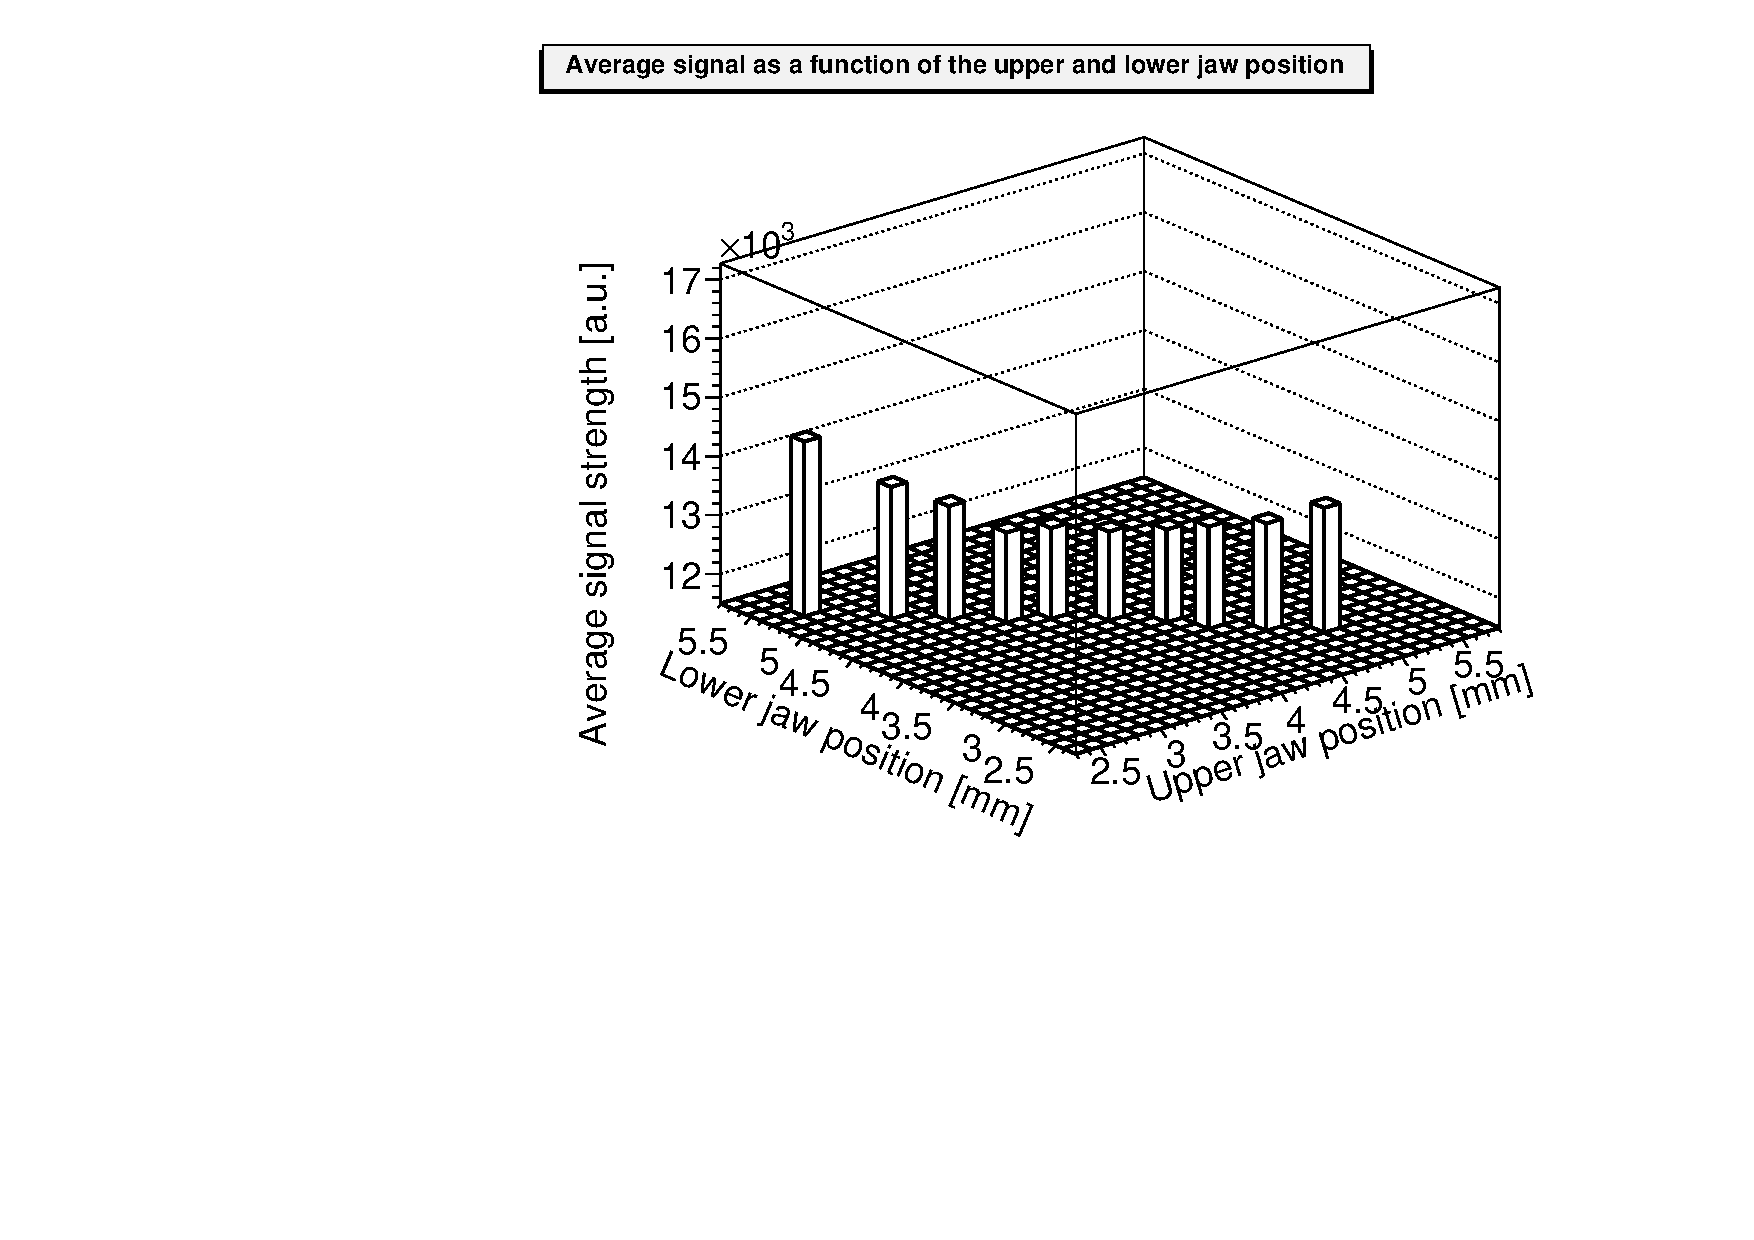
\includegraphics[width=\textwidth]{AsymmetricScan_4mm_beamintensity101_lego.pdf}
\end{subfigure}
\begin{subfigure}[b]{0.5\textwidth}
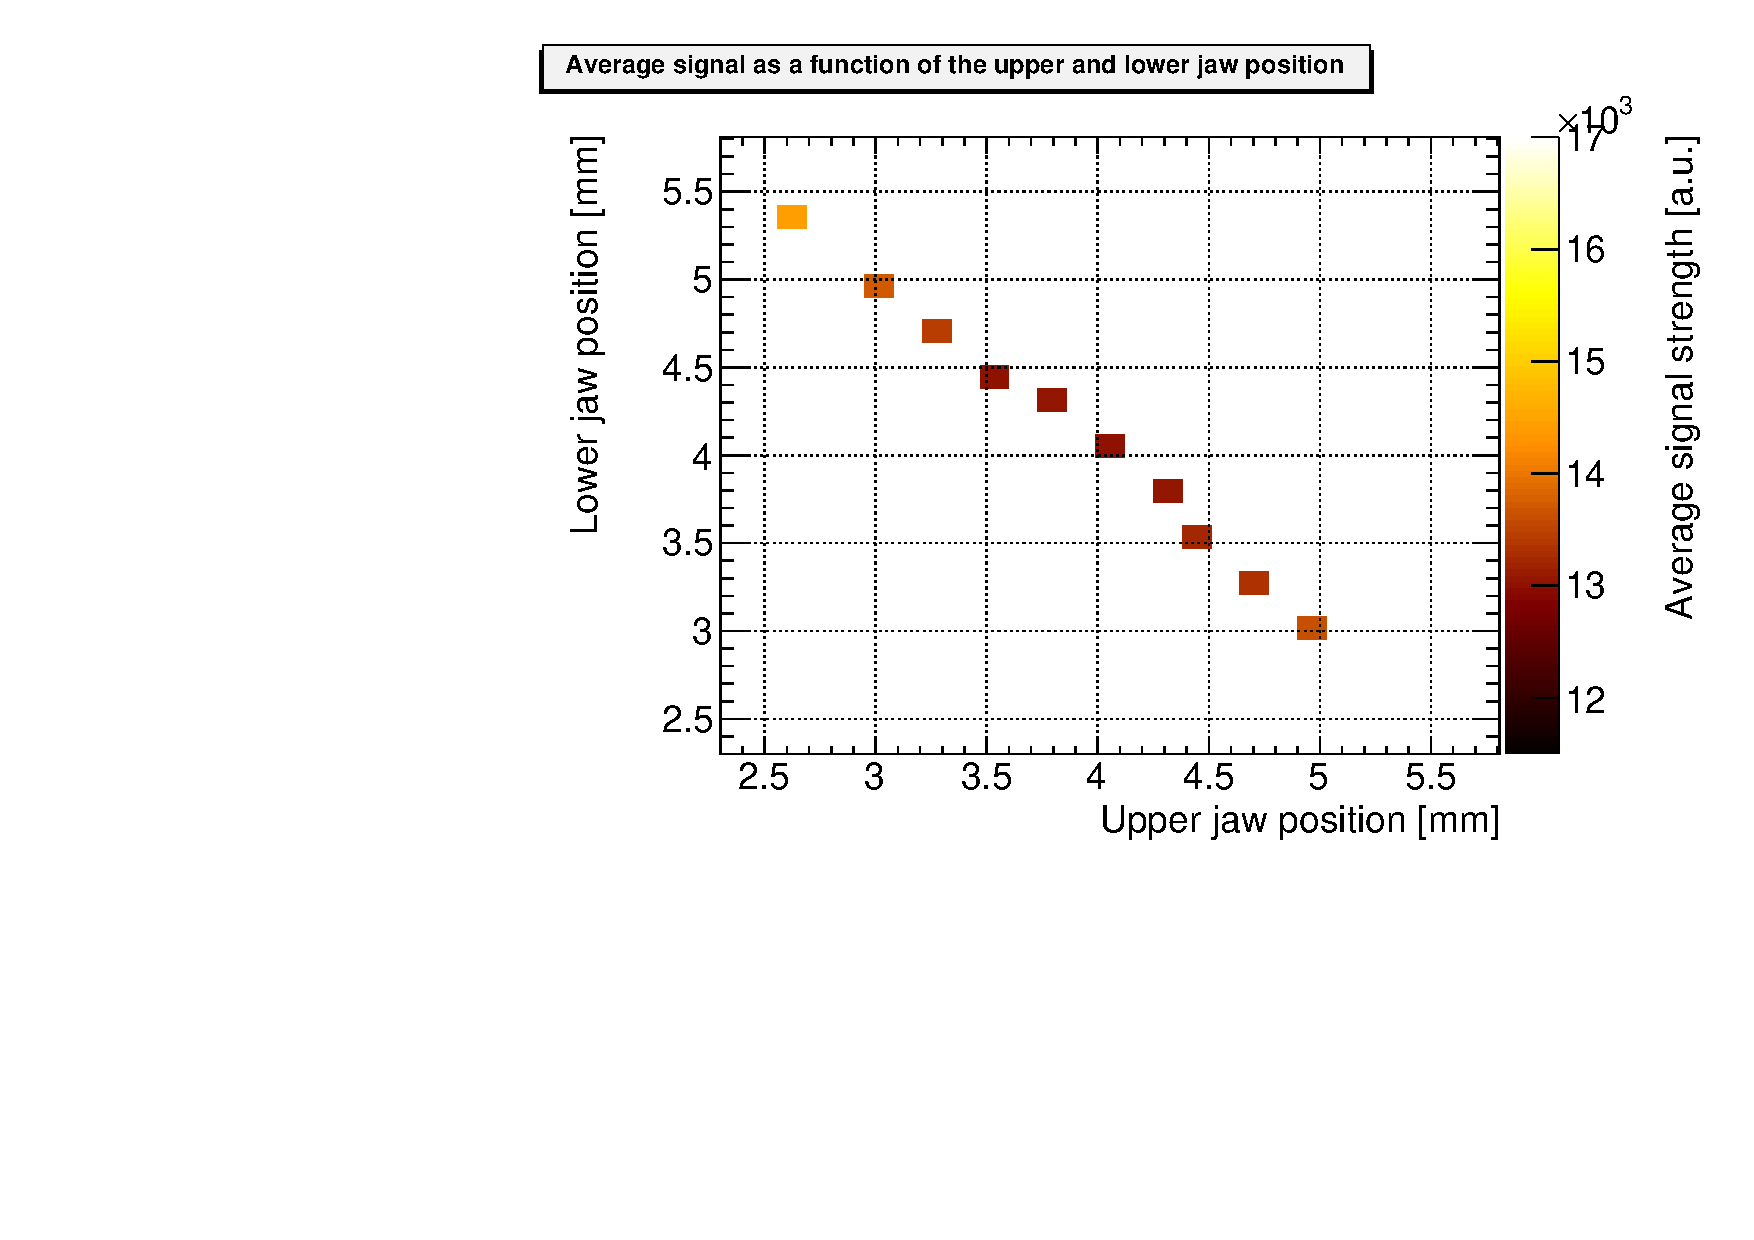
\includegraphics[width=\textwidth]{AsymmetricScan_4mm_beamintensity101_colz.pdf}
\end{subfigure}
\caption[RHUL Cherenkov detector signal for certain upper/lower jaw positions around \SI{4}{\milli\metre}, for a beam intensity of \num{1.01}$\pm$\num{0.03e10}]{Average signal as a function of the position of the upper and lower jaw of the vertical beam halo collimator. The signal was measured for a beam intensity of \num{1.01}$\pm$\num{0.03e10} and a PMT voltage of \SI{900}{\volt}. The jaws were moved simultaneously around \SI{4}{\milli\metre}. For each jaw position, at least 500 ADC pulses were recorded, and the signal was averaged over the number of pulses. The content of the bins were set to the appropriate average signal strength at that point.}
\label{fig:AverageSignal_Asymmetric_4mm_101}
\end{figure}
\begin{figure}
\begin{subfigure}[b]{0.5\textwidth}
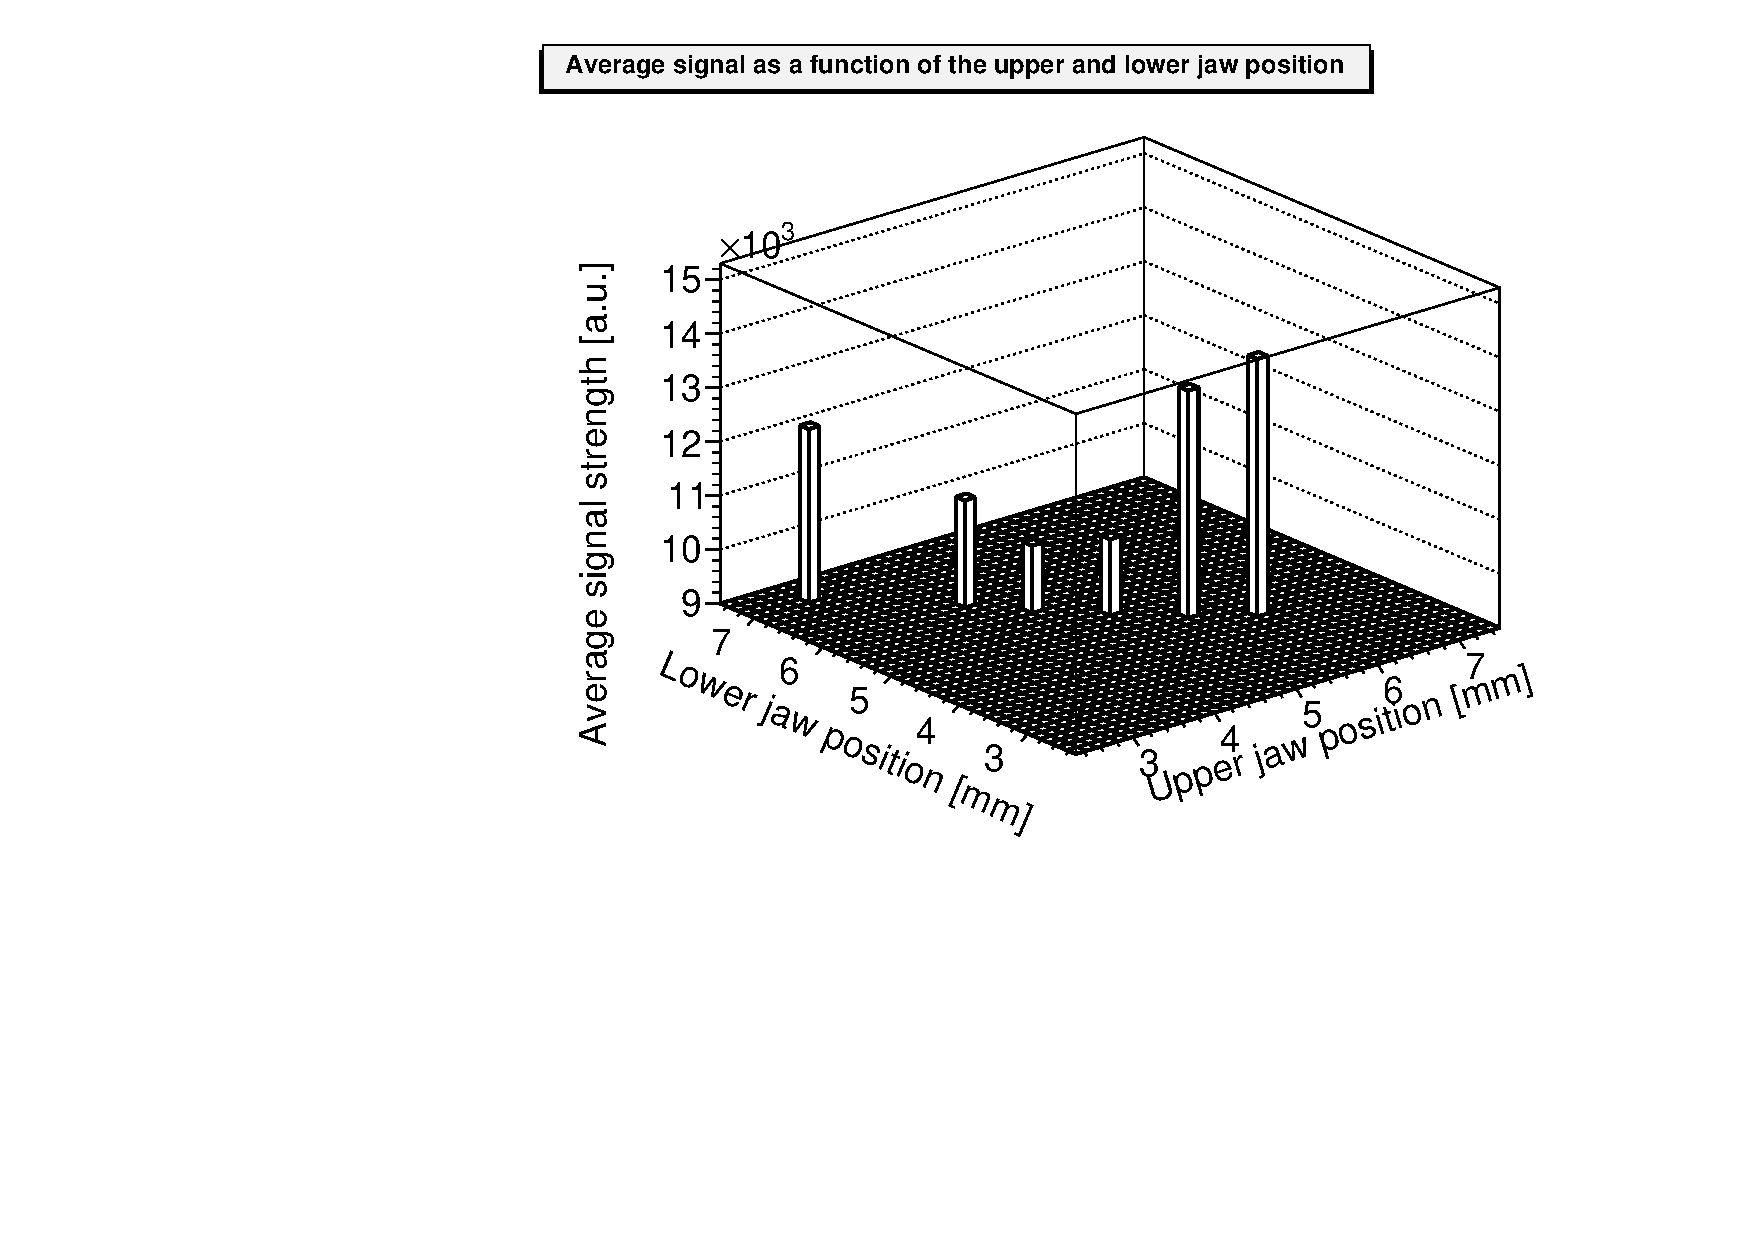
\includegraphics[width=\textwidth]{AsymmetricScan_5mm_beamintensity084_lego.pdf}
\end{subfigure}
\begin{subfigure}[b]{0.5\textwidth}
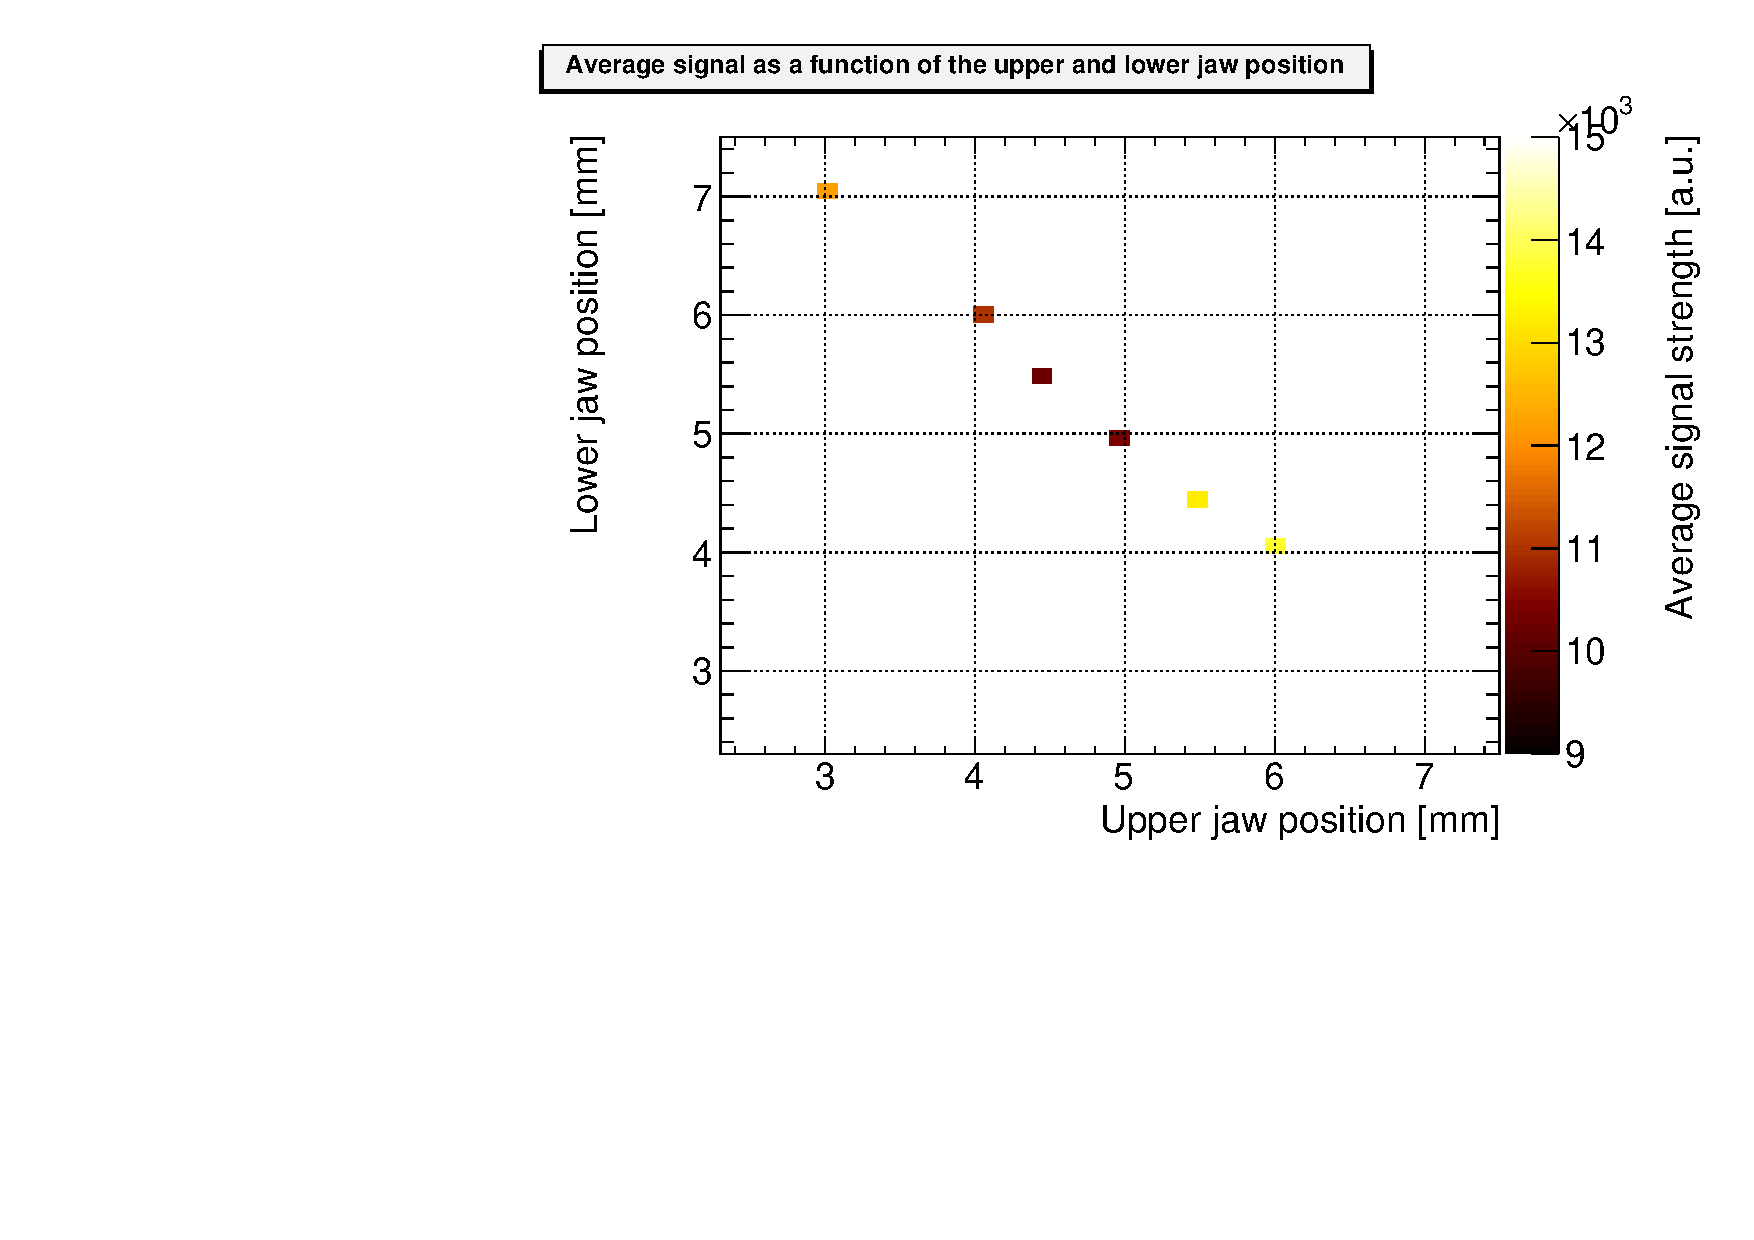
\includegraphics[width=\textwidth]{AsymmetricScan_5mm_beamintensity084_colz.pdf}
\end{subfigure}
\caption[RHUL Cherenkov detector signal for certain upper/lower jaw positions around \SI{5}{\milli\metre}, for a beam intensity of \num{0.84}$\pm$\num{0.03e10}]{Average signal as a function of the position of the upper and lower jaw of the vertical beam halo collimator. The signal was measured for a beam intensity of \num{0.84}$\pm$\num{0.03e10} and a PMT voltage of \SI{900}{\volt}. The jaws were moved simultaneously around \SI{5}{\milli\metre}. For each jaw position, at least 500 ADC pulses were recorded, and the signal was averaged over the number of pulses. The content of the bins were set to the appropriate average signal strength at that point.}
\label{fig:AverageSignal_Asymmetric_5mm_084}
\end{figure}
\begin{figure}
\begin{subfigure}[b]{0.5\textwidth}
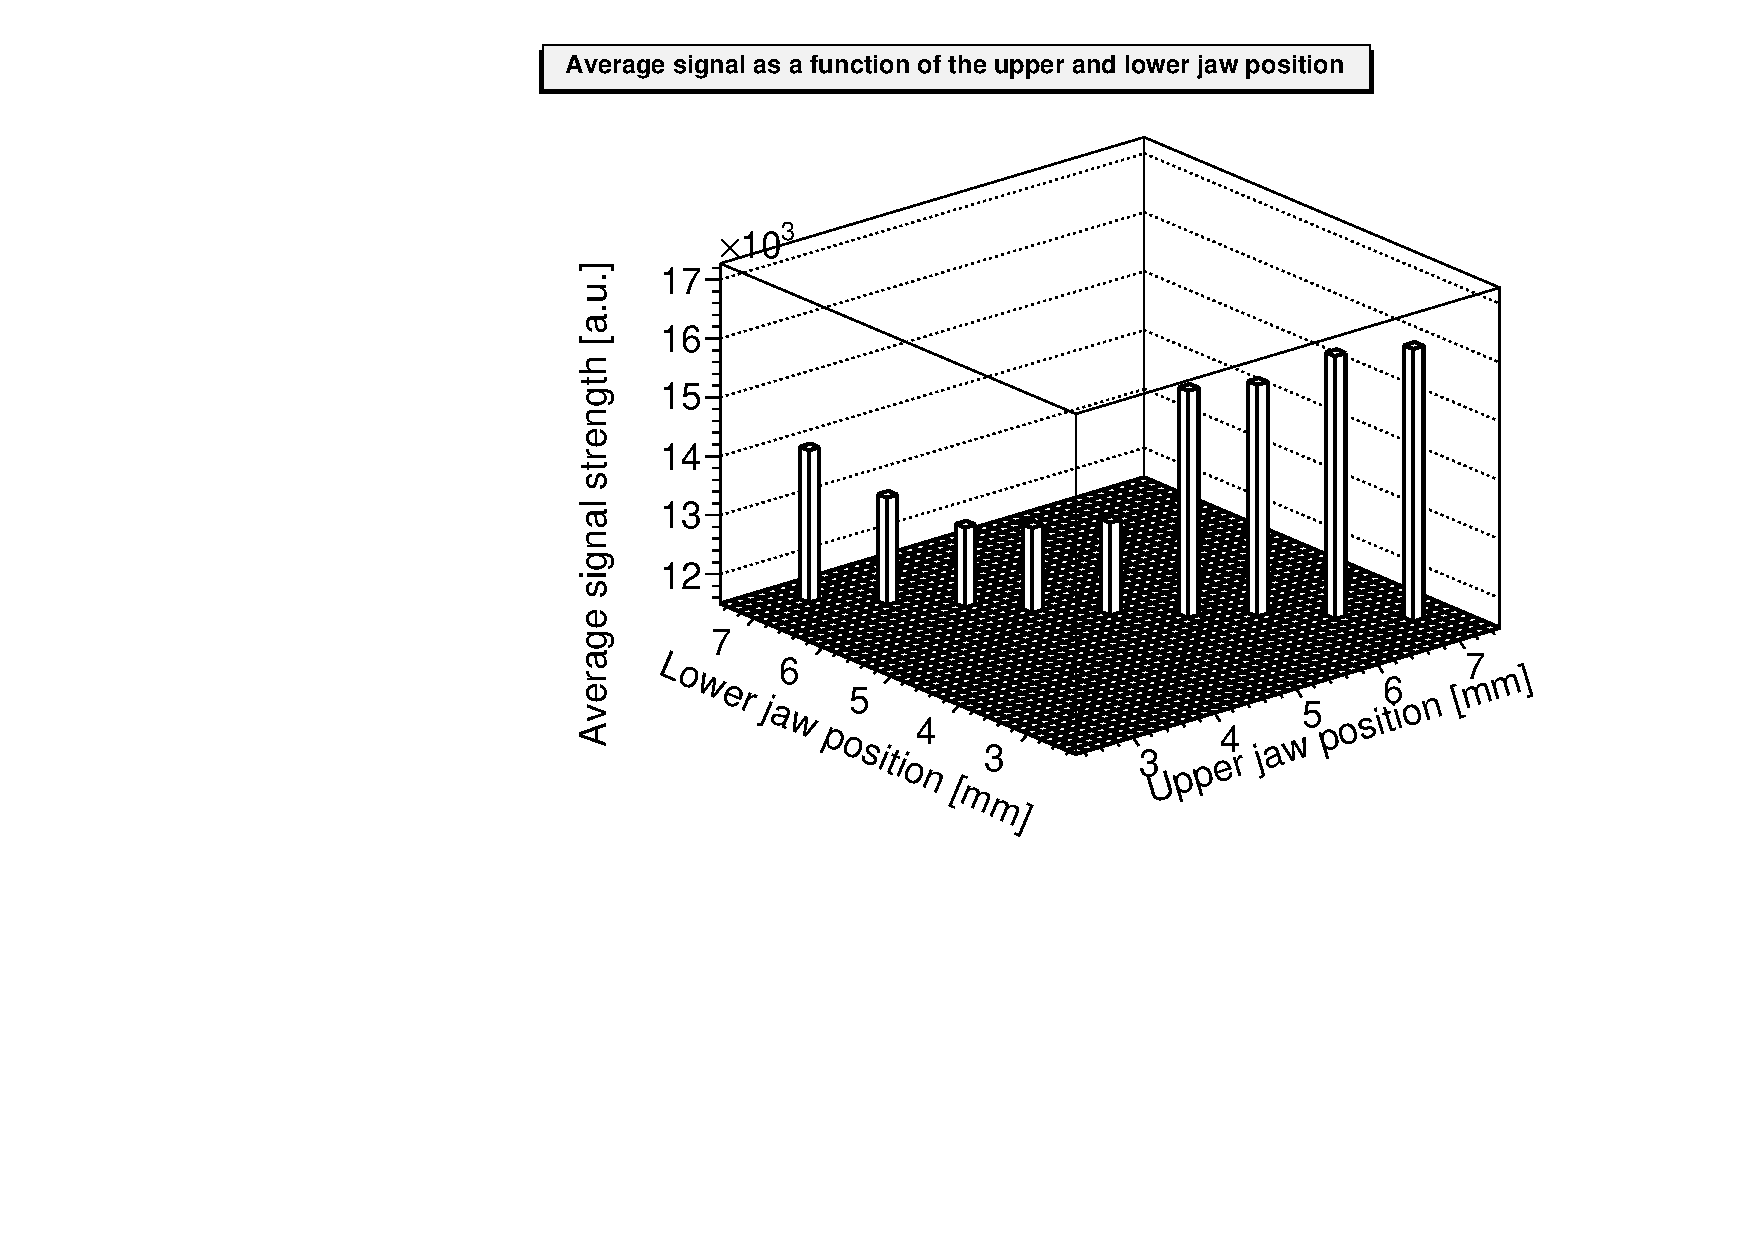
\includegraphics[width=\textwidth]{AsymmetricScan_5mm_beamintensity101_lego.pdf}
\end{subfigure}
\begin{subfigure}[b]{0.5\textwidth}
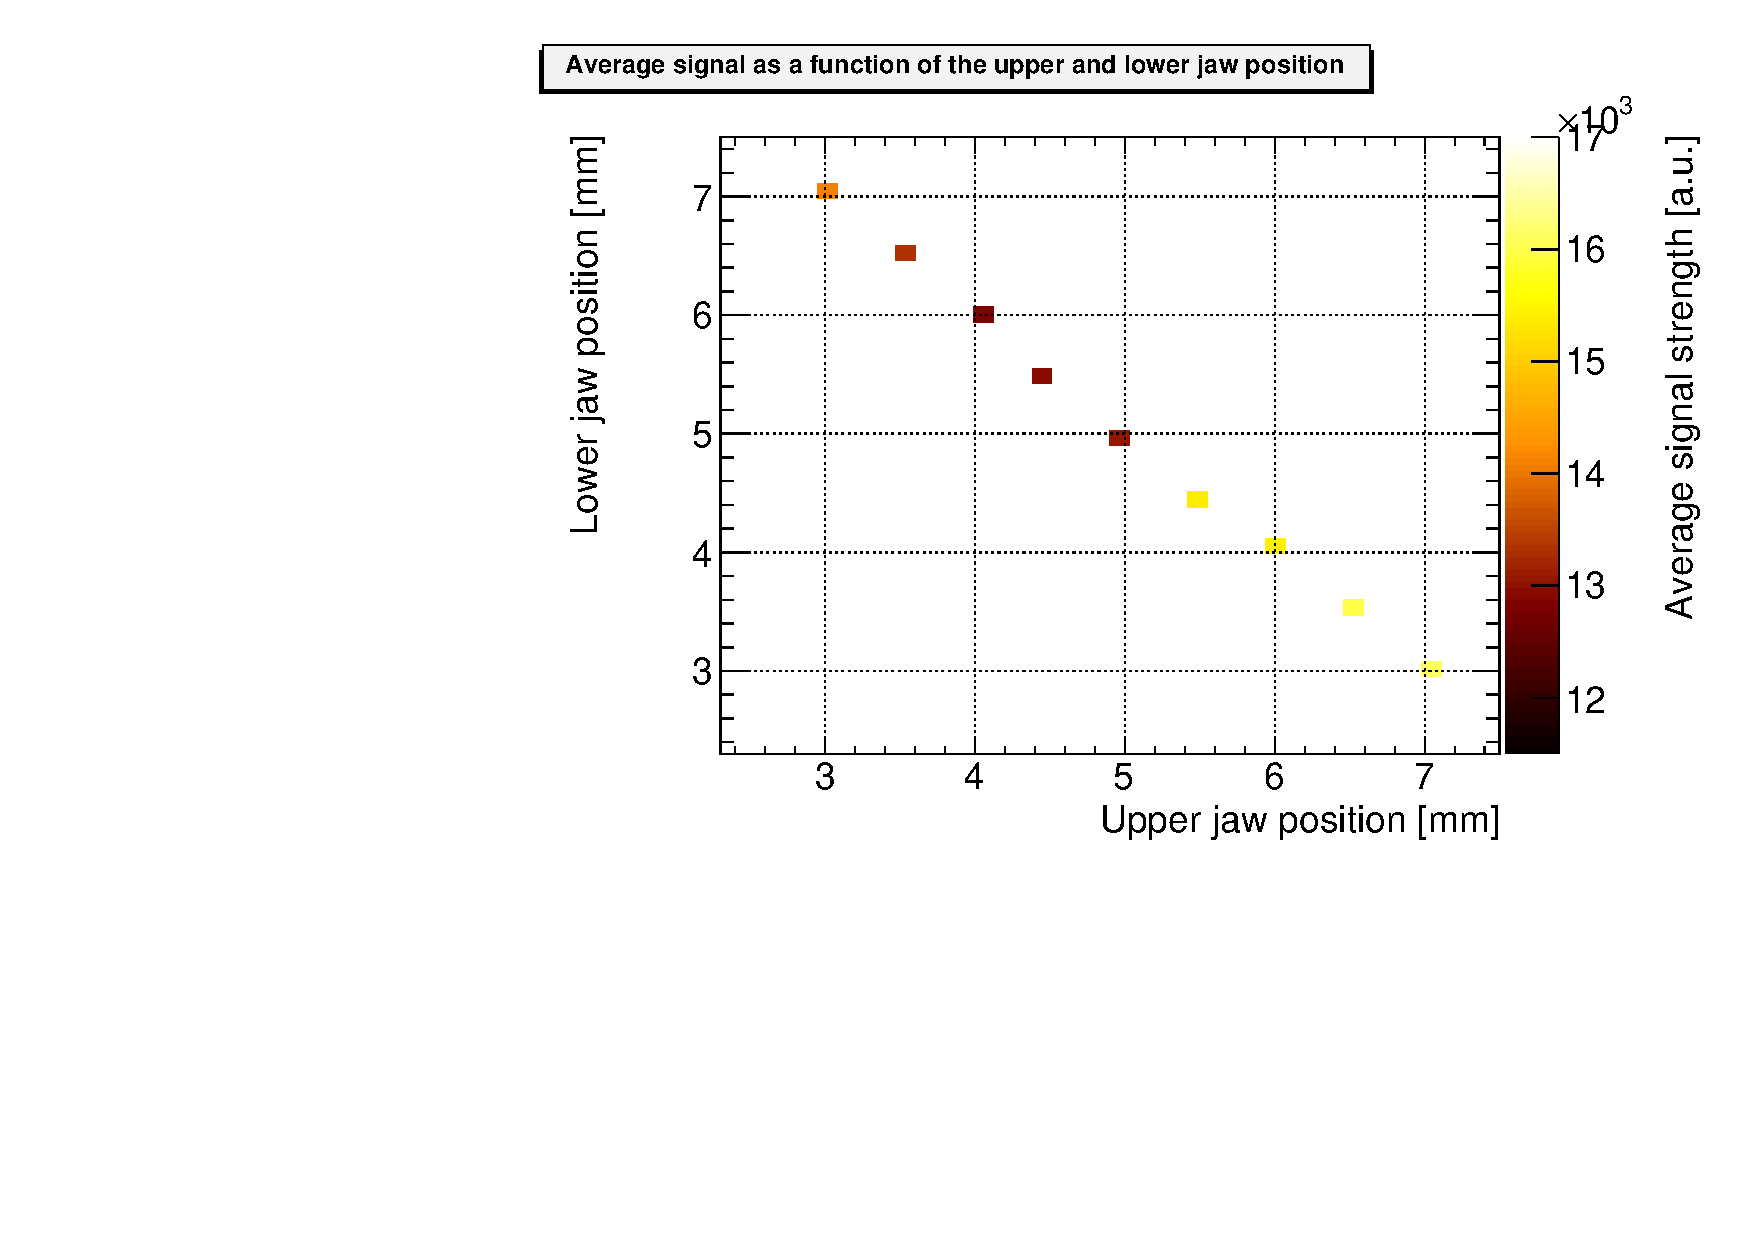
\includegraphics[width=\textwidth]{AsymmetricScan_5mm_beamintensity101_colz.pdf}
\end{subfigure}
\caption[RHUL Cherenkov detector signal for certain upper/lower jaw positions around \SI{5}{\milli\metre}, for a beam intensity of \num{1.01}$\pm$\num{0.03e10}]{Average signal as a function of the position of the upper and lower jaw of the vertical beam halo collimator. The signal was measured for a beam intensity of \num{1.01}$\pm$\num{0.03e10} and a PMT voltage of \SI{900}{\volt}. The jaws were moved simultaneously around \SI{5}{\milli\metre}. For each jaw position, at least 500 ADC pulses were recorded, and the signal was averaged over the number of pulses. The content of the bins were set to the appropriate average signal strength at that point.}
\label{fig:AverageSignal_Asymmetric_5mm_101}
\end{figure}
%---------------------------------------------------
\subsection{Collimator as background source}
\label{sec:BDSIM_sim}
As the data in the figures in the two previous sections have shown, the collimator reduces the existing background level if closed to an aperture of \SI{10}{\milli\metre}. By closing the jaws further, the background level increases again. The questions where this already existing background is coming from, and how the background is increased by the jaws driven into the beam, are now addresses by the following plots showing data from \bdsim simulations of the ATF2 lattice.

\subsection{Effect on background level at IP}
\label{collimator_bkg_IP}
We have seen that the background level around the collimator area is dramatically affected by the movement of the collimator jaws. However, the actual effect of the collimator on the background level at the interaction point might be different, and is now discussed.

%---------------------------------------------------
\section{Background from a Muon Spoilers}
\subsection{MUCARLO}
